%%%%%%%%%%%%%%%%%%%%%%%%%%%%%%%%%%%%%%%%%%%%%%%%%%%%%%%%%%%%%%%%%%%%%%%%%%% 
% Nombre del trabajo, 
% titulo,
% autores
% fechas, 
% comentarios, etc.
%
%%%%%%%%%%%%%%%%%%%%%%%%%%%%%%%%%%%%%%%%%%%%%%%%%%%%%%%%%%%%%%%%%%%%%%%%%%% 
%\input includes/miscomandos.tex % Comandos definidos por el autor

%\documentclass[a4paper,twoside,12pt]{book} 
\documentclass[12pt,a4paper,twoside]{book} 

% Incluir los paquetes necesarios 
\usepackage{setspace}
\usepackage[utf8]{inputenc} % Caracteres con acentos. 
\usepackage[spanish]{babel}
\usepackage[top=4cm, bottom=4cm, left=4cm, right=2.5cm]{geometry}%Para mrgenes
\usepackage{listings}
\usepackage{color}
\usepackage{tabularx}
\usepackage{listings}
\usepackage{latexsym} % Simbolos 
\usepackage[pdftex=true,colorlinks=true,linkcolor=black,plainpages=false]{hyperref}
\usepackage[pdftex]{graphicx} %Inclusin de graficos PDFLaTeX
\DeclareGraphicsExtensions{.png,.pdf,.jpg}
\usepackage{pdfpages}
\usepackage{wrapfig}
\usepackage{float}
\usepackage{lscape} 
\usepackage{xr}%Referencias a otros documentos
\usepackage{subfigure}
\externaldocument{subversion}

\setcounter{secnumdepth}{3} 
\setcounter{tocdepth}{3} 

% Define colors
\definecolor{MyLightMagenta}{cmyk}{0.1,0.8,0,0.1}
\definecolor{MyDarkBlue}{rgb}{0.1,0,0.55}

\hypersetup{urlcolor=blue} 
\hypersetup{colorlinks,urlcolor=blue} 
 
\lstset{
 language=C++,
 basicstyle=\footnotesize,
 keywordstyle=\color{blue}\bfseries,
 identifierstyle=\ttfamily,
 % commentstyle=\itshape,
 stringstyle=\color{MyDarkBlue},
 showstringspaces=false,
 numbers=left,
 numberstyle=\ttfamily,
 stepnumber=1,
 tabsize=2,
 breaklines=true,
 numbersep=5pt,
 xleftmargin=15pt,
 frame=leftline,
 mathescape=true,
 breaklines=false, 
 escapeinside={(*@}{@*)},
 escapechar=\ç
 }
 
\clubpenalty=1000
\widowpenalty=1000
\newlength{\codeindent}
\setlength{\codeindent}{.2cm}
\newcommand{\code}[2]{%
  \fontfamily{pcr}\fontsize{8}{8}\selectfont
  \setlength{\baselineskip}{1pt}
  %\arabic{codeline}\hspace{#1\codeindent}{#2}
  \hspace{#1\codeindent}{#2}
%  \stepcounter{codeline}
}

% Titulo, autor(es), fecha. 
\title{Dosier RenegadeKlingon}
\author{Angel Baltar Diaz} 
\date{\Large Agosto, 2013} 
\renewcommand{\baselinestretch}{1.5} 
\renewcommand{\tablename}{Tabla} 
\renewcommand{\listtablename}{Indice de tablas} 

\newcommand{\scvar}[1]{{\tt {#1}}}

\begin{document} 
%portada
%\input miscomandos.tex % Comandos definidos por el autor

%\documentclass[a4paper,12pt]{book} 

% Incluir los paquetes necesarios 
%\usepackage[latin1]{inputenc} % Caracteres con acentos. 
%\usepackage[spanish]{babel}
%\usepackage{latexsym} % Smbolos 
%\usepackage[pdftex=true,colorlinks=true,plainpages=false]{hyperref} % Soporte hipertexto
%\usepackage[pdftex]{graphicx} %Inclusin de grficos PDFLaTeX
%\usepackage{color}
%\DeclareGraphicsExtensions{.png,.pdf,.jpg}
%\sloppy % suaviza las reglas de ruptura de lneas de LaTeX
%\renewcommand{\baselinestretch}{1.5} %espacio entre lineas
%\pagestyle{empty}

% Ttulo, autor, fecha. 
\title{portada} 
\author{Angel Baltar Diaz}
\date{\Large Enero, 2013} 

%\begin{document}
\begin{titlepage}
\begin{figure}
\begin{center}

\includegraphics[width=5cm]{includes/images/logo.png}
\\ {\large Dosier RenegadeKlingon}
\\[3cm]
\end{center}
\end{figure}
\begin{center}
{\Large with2balls}

\end{center}
\begin{flushright}
{\large Autor: Angel Baltar Diaz}
\end{flushright}
\end{titlepage}
%\end{document}
\newpage{\pagestyle{empty}\cleardoublepage}
%
\includepdf{includes/pagina_blanco.pdf}
%
\includepdf{includes/pagina_blanco.pdf}
%
\includepdf{pagina_blanco.pdf}


\tableofcontents % Tabla de contenido 
\newpage 
\listoffigures % indice de figuras 

%Capitulo 1
%%%%%%%%%%%%%%%%%%%%%%%%%%%%%%%%%%%%%%%%%%%%%%%%%%%%%%%%%%%%%%%%%%%%%%%%%%% 
% Nombre del trabajo, 
% t�tulo,
% autores
% fechas, 
% comentarios, etc.
%%%%%%%%%%%%%%%%%%%%%%%%%%%%%%%%%%%%%%%%%%%%%%%%%%%%%%%%%%%%%%%%%%%%%%%%%%% 
%\input miscomandos.tex % Comandos definidos por el autor

%\documentclass[a4paper,12pt]{book} 

%% Incluir los paquetes necesarios 
%\usepackage[latin1]{inputenc} % Caracteres con acentos. 
%\usepackage[spanish]{babel}
%\usepackage{latexsym} % Simbolos 
%\usepackage[pdftex=true,colorlinks=true,plainpages=false]{hyperref} % Soporte hipertexto
%\usepackage[pdftex]{graphicx} %Inclusión de gr�ficos PDFLaTeX
%\DeclareGraphicsExtensions{.png,.pdf,.jpg}
%\renewcommand{\baselinestretch}{1.5} %espacio entre lineas
%\sloppy % suaviza las reglas de ruptura de l�neas de LaTeX

% T�tulo, autor, fecha. 
\title{capitulo1} 
\author{Angel baltar Diaz}
\date{\Large Enero, 2010} 

%\begin{document} % Inicio del documento
%capitulo 1 introduccion
\chapter {El juego}
\label{capitulo1}

En este capítulo presentaremos el juego, su temática, estilo y cual es la concepción general del título, que es lo que hace hasta el momento y cuales son en general las líneas de trabajo que están planteadas.

\section{Temática del juego}

Este juego se basa en la típica temática de guerra entre naves espaciales, es un juego estilo R-type en el que el jugador maneja una única nave y debe destruir ejércitos enteros de naves enemigas, dentro de este estilo de juego la temática en si está abierta, no hay una historia concreta en la que el juego se base por el momento.

Se ha planteado desde un principio una temática basada en el universo star Trek en el que el protagonista es un klingon que toma una nave por su cuenta y se lanza a conquistar territorios enemigos, sin embargo como ya decía la temática esta completamente abierta mientras se mantenga el estilo de juego. Si en algun momento se quiere prescindir de la temática basada en star trek por temas de licencias o por cualquier otro motivo, no habría problema en hacerlo, además tecnicamente es simplemente cambiar imágenes de naves, fondos de los escenarios, logos etc. 

\begin{figure}[t]
\centering
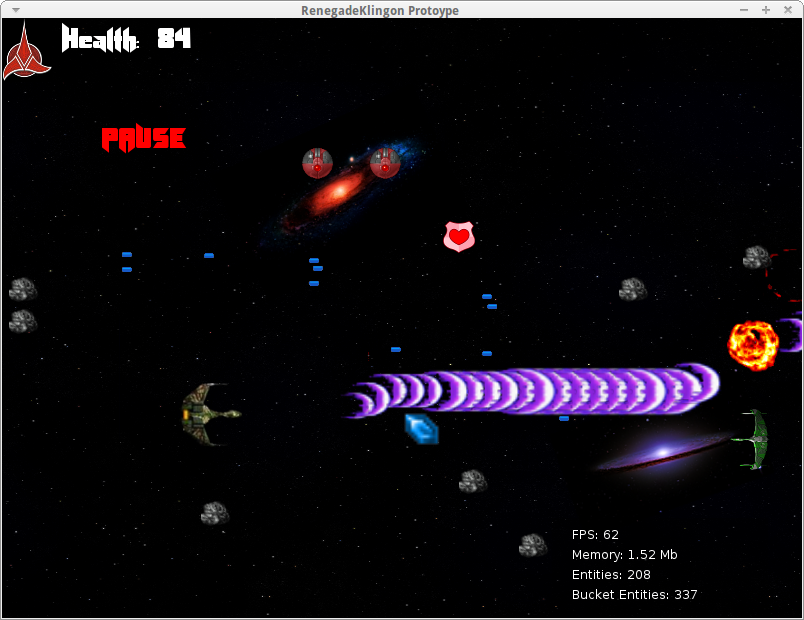
\includegraphics[width=\linewidth]{includes/images/Screen_Shoot1.png}
\caption{Captura de pantalla del juego}
\label{fig:RenegadeKlingonScreenShoot}
\end{figure}


%section objetivos
\section{Objetivos}

Este juego surje como un simple hobby, he estado dedicando tiempo libre a su construcción, en general las partes de programación no me plantean excesivos problemas, sin embargo tengo lagunas muy importantes en el apartado gráfico porque no sé lo suficiente de diseño gráfico.
Tal como he planteado el juego los objetivos que tengo para el son los siguientes:

\begin{itemize}
\item Juego en 2d estilo \textbf{R-type}[\ref{glosario}].
\item Niveles diseñables y extensibles sin necesidad de programar (basados en generación mediante Tiled).
\item Armas intercambiables que se puedan ir consiguiendo durante el juego.
\item Sistema de juego basado en nivel de salud combinable con número de vidas.
\item Soporte como aplicación de escritorio para Mac, Windows y linux
\item Soporte para dispositivos móviles
\item Soporte para jugar a través de Web
\end{itemize}

Algunos de estos objetivos están actualmente cumplidos, otros son en principio tecnicamente viables y de otros simplemente aun no he mirado como pueden hacerse, en otros capítulos entraremos más en detalles técnicos sobre todas estas cuestiones.

%\end{document} % Fin del documento

%Capitulo 2
%%%%%%%%%%%%%%%%%%%%%%%%%%%%%%%%%%%%%%%%%%%%%%%%%%%%%%%%%%%%%%%%%%%%%%%%%%% 
% Nombre del trabajo, 
% t�tulo,
% autores
% fechas, 
% comentarios, etc.
%%%%%%%%%%%%%%%%%%%%%%%%%%%%%%%%%%%%%%%%%%%%%%%%%%%%%%%%%%%%%%%%%%%%%%%%%%% 
%\input miscomandos.tex % Comandos definidos por el autor

%\documentclass[a4paper,12pt]{book} 

%% Incluir los paquetes necesarios 
%\usepackage[latin1]{inputenc} % Caracteres con acentos. 
%\usepackage[spanish]{babel}
%\usepackage{latexsym} % Simbolos 
%\usepackage[pdftex=true,colorlinks=true,plainpages=false]{hyperref} % Soporte hipertexto
%\usepackage[pdftex]{graphicx} %Inclusión de gr�ficos PDFLaTeX
%\DeclareGraphicsExtensions{.png,.pdf,.jpg}
%\renewcommand{\baselinestretch}{1.5} %espacio entre lineas
%\sloppy % suaviza las reglas de ruptura de l�neas de LaTeX

% T�tulo, autor, fecha. 
\title{capitulo2} 
\author{Angel baltar Diaz}
\date{\Large Enero, 2010} 

%\begin{document} % Inicio del documento
%capitulo 1 introduccion
\chapter {Consideraciones técnicas}
\label{capitulo2}

En este capítulo hablaremos sobre como se encuentra tecnicamente el juego, repasaremos los objetivos planteados en el capítulo anterior y sobre cada uno evaluaremos su estado.

\section{Juego 2d estilo R-type}

Este objetivo es el principal del juego, es el corazón del mismo, conseguir un estilo de juego 2d con una jugabilidad similar a la de los clásicos R-type.

Para conseguir este objetivo ha tenido que programarse el framework base del videojuego, este se basa en una clase llamada Space que no es mas que un simulador del espacio en el que se desrrolla la acción, es decir controla diversas acciones como son:

\begin{itemize}

\item Actualización de todos los objetos del escenario en cada frame.

\item Sistema de colisiones entre objetos, decide si por ejemplo una bala debe colisionar con una nave provocando una explosión. El sistema de colisiones esta basado en Buckets para mayor rendimiento.

\item Dibujado de todos los objetos en el escenario, incluyendo soporte para \textbf{parallax} [\ref{glosario}] en varios niveles o planos. Este soporte está implementado actualmente pero es bastante mejorable.

\item Control de objetos fuera de límite del escenario

\item Control de la aparición de objetos al desplazarse el jugador hacia adelante en el mapa

\end{itemize}

Todo este framework esta actualmente construido y funcionando, no obstante como es el núcleo fundamental del juego esta sujeto a cambios frecuentes, y dependiendo de la dirección en la que se realice el trabajo futuro tendra que ser actualizado, para la implementación de nuevas funcionalidades, temás de rendimiento etc.

\section{Niveles diseñables y extensibles}

Uno de los objetivos planteados desde un principio es que los niveles o fases del juego no vayan directamente programados, sino que sean archivos que el juego sea capaz de cargar. Esto supone una tremenda ventaja ya que el juego se hace extensible por definición simplemente añadiendo más mapas o niveles, no obstante también tiene desventajas como cierta pérdida de flexibilidad al tener que pensar todos los objetos y demás de forma que puedan ser diseñados y cargados en mapas.

El sistema de mapas está actualmente ya implementado, lo que se refiere al soporte básico, el mayor trabajo que falta en el juego y que afecta a los mapas es basicamente implementar cada vez más y más enemigos, armas, minas, y en general objetos cargables desde mapa, para que los diseñadores de niveles del juego tengan un amplio avanico de posibilidades al diseñar sus mapas.

El diseño de mapas se basa en un programa llamado \textbf{Tiled} \url{http://www.mapeditor.org/}.
Este programa se basa en una serie de imágenes (Sprites) y en su combinación en celdas para generar los mapas, realmente lo que se genera es un archivo XML que posteriormente el juego cargará cargando con el las imágenes asociadas.

En RenegadeKlingon existe una manera particular de generar los mapas, las imágenes aplicadas en Tiled no son directamente las cargadas por el juego, sino que existen 2 imágenes, una para el diseño de los mapas y otra que es la que el juego cargará finalmente y que va asociada a la primera y representa lo mismo. Por este motivo los diseñadores de mapas, deben probarlos sobre el juego para darlos por finalizados ya que puede que algunas zonas del mapa no queden en el juego tal como se ven en Tiled.

Esta forma de trabajar esta motivada por algunos problemas técnicos que surjen al cargar objetos que ocupan mas de un \textbf{tile}[\ref{glosario}]

\begin{figure}[t]
\centering
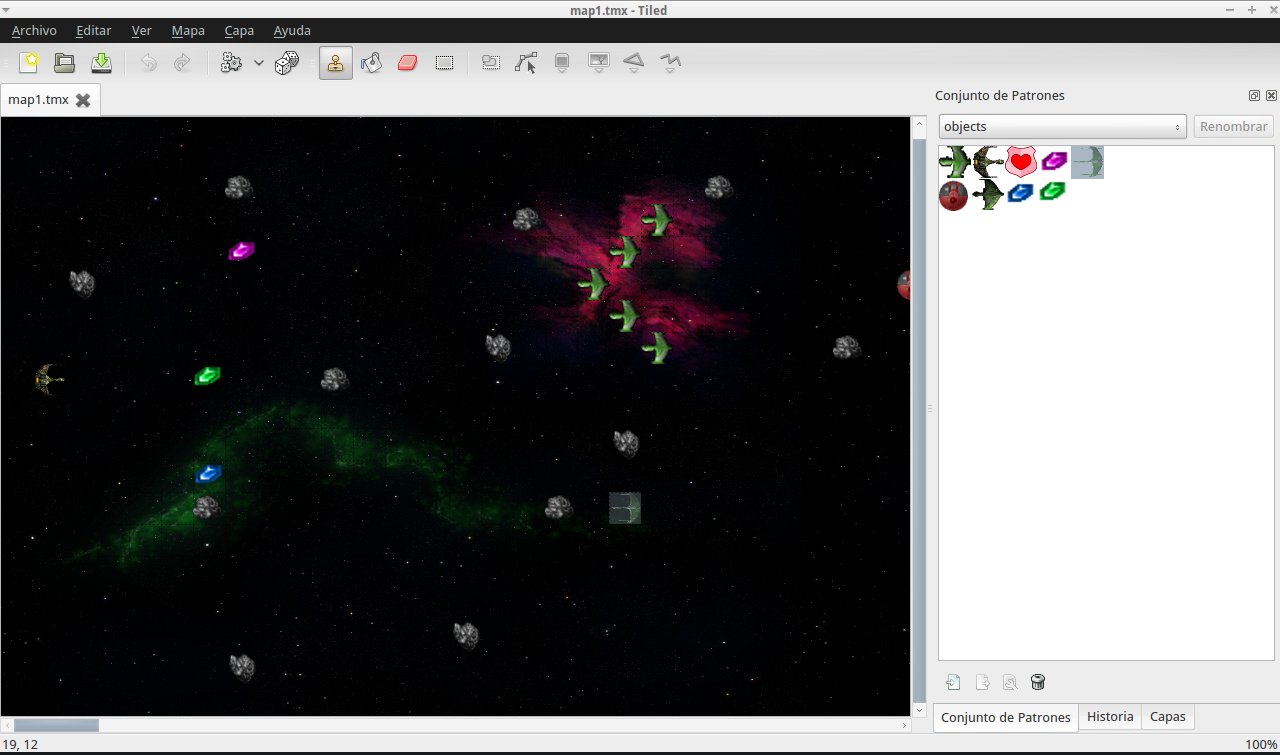
\includegraphics[width=\linewidth]{includes/images/tiled.png}
\caption{Captura de pantalla del programa de generación de mapas}
\label{fig:TiledScreenShoot}
\end{figure}

\section{Sistema de juego basado en nivel de salud y número de vidas}

Actualmente está implementado un sistema de juego basado en nivel de salud, que se decrementa con los disparos recibidos o en general colisiones y puede incrementarse al recoger objetos de salud, no está implementado un sistema basado en número de vidas, pero su implementación sería relativamente sencilla y abordable rapidamente.

\section{Desplegado de la aplicación sistemas soportados y sistemas objetivo}

Actualmente el juego se despliega sobre tres sistemas, Mac, windows y linux, para estos tres sistemas el juego es una simple aplicación de escritorio.Se detalla para cada plataforma:

\begin{itemize}

\item Mac: Tras el correcto empaquetado se proporciona un .app que tras instalarse da acceso al juego.

\item Windows:  Tras el correcto empaquetado se proporciona un .exe que es el ejecutable del juego.

\item Linux: Tras un simple empaquetado se proporciona un .love que ejecutado por la aplicacion para linux love2d ejecutará el juego.

\end{itemize}

Existe además un sistema de despliegue automático basado en un script shell que basicamente se encarga de las siguientes tareas:

\begin{itemize}

\item Empaquetado del juego para cada plataforma

\item Subir cada empaquetado a github en el repositorio llamado RenegadeKlingonDeploy: Para cada plataforma se sube sobre un branch independiente

\item Hacer merge entre los branches de cada plataforma y subir dicho merge sobre el branch master para ofrecer la posibilidad de descargar el juego para las tres plataformas a la vez.

\end{itemize}

Tener el sistema de despliegue automatizado supone una gran ventaja ya que si realizamos cualquier cambio sobre el juego podemos desplegar dicho cambio inmediatamente, y la gente que a partir de ese momento se descargue el juego tendra el último cambio que hemos añadido.

Migrar el juego a Mac y Windows ha sido relativamente sencillo, simplemente son cuestiones de como empaquetar el entregable final que maneja el script comentado anteriormente. Las siguientes plataformas objetivo son dispositivos móviles y desplegado directamente sobre web para ser jugado online, detallamos a continuación ciertas ideas técnicas sobre como llevar a cabo estas migraciones:

\begin{itemize}

\item Android: En principio, pensaba estudiar el proyecto love-native-android \url{https://github.com/hagish/love-native-android}. Muy probablemente habría que mejorar el juego en temas de resolución de pantalla y puede que aparecieran bugs al jugar sobre android. Además habría que estudiar temas de licencia y leer con detalle la licencia del proyecto love-native-android.

\item Iphone: Por el conocimiento que tengo hasta ahora no es técnicamente viable, no hay proyectos que migren automaticamente, y por las discusiones en foros hacer un proyecto a tal fin es una tarea muy compleja.Para llegar a Iphone podrían plantearse vias alternativas como jugar via web

\item Web: Existe un proyecto llamado love-webplayer \url{https://github.com/ghoulsblade/love-webplayer/wiki} que pretende ser un player de love2d sobre javascript, si ese proyecto funciona seria sencillo poner disponible el proyecto via web, también existe algun proyecto similar pero sobre html5, simplemente habria que estudiar estos proyectos y ver cual funciona mejor con el juego.

\end{itemize}
%\end{document} % Fin del documento
%Capitulo 3
%%%%%%%%%%%%%%%%%%%%%%%%%%%%%%%%%%%%%%%%%%%%%%%%%%%%%%%%%%%%%%%%%%%%%%%%%%%% 
% Nombre del trabajo, 
% título,
% autores
% fechas, 
% comentarios, etc.
%%%%%%%%%%%%%%%%%%%%%%%%%%%%%%%%%%%%%%%%%%%%%%%%%%%%%%%%%%%%%%%%%%%%%%%%%%% 
%\input miscomandos.tex % Comandos definidos por el autor

%\documentclass[a4paper,12pt]{book} 

%% Incluir los paquetes necesarios 
%\usepackage[latin1]{inputenc} % Caracteres con acentos. 
%\usepackage[spanish]{babel}
%\usepackage{latexsym} % Simbolos 
%\usepackage[pdftex=true,colorlinks=true,plainpages=false]{hyperref} % Soporte hipertexto
%\usepackage[pdftex]{graphicx} %Inclusión de gráficos PDFLaTeX
%\DeclareGraphicsExtensions{.png,.pdf,.jpg}
%\renewcommand{\baselinestretch}{1.5} %espacio entre lineas
%\sloppy % suaviza las reglas de ruptura de líneas de LaTeX

% Título, autor, fecha. 
\title{capitulo4} 
\author{Angel Baltar Diaz}
\date{\Large Enero, 2013} 

%\begin{document} % Inicio del documento
%capitulo 4 LLVM
\chapter {Fundamentos teóricos}
\label{capitulo3}

En este capítulo explicaremos las principales características, partes y funcionamiento del compilador LLVM, que es el utilizado en el desarrollo de este proyecto. También haremos una breve introducción para explicar conceptos básicos de compilación.

\section{Infraestructura de compilación LLVM:}

\subsection{Introducción a los compiladores}
Vamos a explicar algunos términos que serán de ayuda para la comprensión del funcionamiento de LLVM. 
Además de los aquí explicados, sería de gran ayuda revisar las definiciones de los términos AST, CFG, DDG, CG, etc. explicadas en el glosario de términos \{cap.~\ref{glosario}\} 

%------------------------------------------------------------------
%------------------------------------------------------------------
\subsubsection*{Representación Static Single Assignment (SSA)}

En el diseño de compiladores, la representación SSA es una representación intermedia en la cual cada variable se asigna una única vez. Las variables existentes en el código original, en general, son versionadas y sustituidas por nuevas variables que se componen del nombre original y un subíndice de tal manera que cada definición tiene su propia versión. En la representación SSA, las cadenas de uso-definición son explícitas y cada una de ellas contiene un solo elemento.
Un algoritmo para la construcción eficiente de SSA fué desarrollado por Ron Cytron, Jeanne Ferrante, Barry Rosen, Mark Wegman y Ken Zadeck, todos ellos investigadores de IBM en la década de los 80.

\begin{figure}[t]
\begin{center}
\subfigure[Código Fuente]{
  \scalebox{0.7}{\includegraphics{includes/images/ssa_intro_source.pdf}}
\label{fig:ssa_ejemplo1a}
}
\hspace{2em}
\subfigure[Grafo de Control de Flujo (CFG)]{
  \scalebox{0.7}{\includegraphics{includes/images/ssa_intro_1.pdf}}
\label{fig:ssa_ejemplo1b}
}
\caption{Transformación del código fuente de un programa a su representación SSA. Pasos a y b.}
\label{FIG:intro:ssa_ejemplo1}
\end{center}
\end{figure}
%

La transformación de un código fuente en su representación SSA consta básicamente de dos pasos. Primero se reemplaza cada asignación de variable con una nueva variable (nueva versión de variable para ser exactos) y segundo, se reemplaza cada uso de cada variable con la ``versión''  correspondiente que alcanza en ese punto del grafo de control de flujo (CFG). Por ejemplo, consideremos el código fuente de la Figura~\ref{fig:ssa_ejemplo1a} y su correspondiente grafo de control de flujo de la Figura~\ref{fig:ssa_ejemplo1b}. A continuación se crean nuevas variables (p.ej. \scvar{x$_1$} y \scvar{x$_2$}) cada una de las cuales se asigna una única vez y se establecen subíndices para distinguir las referencias de estas variables, obteniendo el código resultante que se muestra en la Figura~\ref{fig:ssa_ejemplo2}.
%
\begin{figure}[t]
\begin{center}
\setcounter{subfigure}{2}
\subfigure[Renombrado de variables]{
  \scalebox{0.7}{\includegraphics{includes/images/ssa_intro_2.pdf}}
\label{fig:ssa_ejemplo2c}
}
%
%\hspace{2em}
\subfigure[Ubicación de nodos $\phi$]{
  \scalebox{0.7}{\includegraphics{includes/images/ssa_intro_3.pdf}}
\label{fig:ssa_ejemplo2d}
}
\caption{Transformación del código fuente de un programa a su representación SSA. Pasos c y d.}
\label{fig:ssa_ejemplo2}
\end{center}
\end{figure}
%
De esta forma se ha establecido la definición que se corresponde con cada uso, excepto para el caso de los usos de la variable \scvar{y} en el último bloque básico del CFG, ya que éstos pueden referirse tanto a \scvar{y$_1$} como a \scvar{y$_2$}, dependiendo de cómo haya transcurrido el flujo de control hasta llegar a ese punto.
Así, con objeto de determinar que definición (\scvar{y$_1$} o \scvar{y$_2$}) alcanza ese punto de confluencia en el grafo de control de flujo del programa, se añaden nuevas sentencias que contienen unos operadores especiales denominados nodos $\phi$. Estos operadores se insertan al comienzo del bloque básico ubicado en el punto de confluencia del CFG. En el ejemplo se crea una nueva sentencia \scvar{y$_3$ = $\phi$(y$_1$, y$_2$)} que da lugar a una nueva definición de la variable \scvar{y}, denominada \scvar{y$_3$} y que recoge las definiciones \scvar{y$_1$} o \scvar{y$_2$} que potencialmente pueden alcanzar ese punto del programa en función de la rama de control que se ejecute.

En la Figura~\ref{fig:ssa_ejemplo2d} se aprecia como los usos de la variable \scvar{y}, en el último bloque básico, referencian directamente la variable \scvar{y$_3$}, obteniéndose siempre el valor correcto. Nótese que para la variable \scvar{x} no es necesario añadir un nuevo operador $\phi$ ya que existe una única definición \scvar{x$_2$} que puede alcanzar el bloque básico ubicado en el punto de confluencia del CFG, independientemente de la rama de control que se ejecute.


%
\subsubsection*{Representación Gated Single Assignment (GSA)}
La representación de programas Gated Single Assignment (GSA) es una extensión de SSA que fué introducida por Balance, Maccabe y Ottenstein como parte de una representación más compleja denominada Program Dependence Web [Arenaz et al. 2008a].
%
%
\begin{figure}[t]
\begin{center}
\scalebox{0.7}{\includegraphics{includes/images/gsa_intro.pdf}}
\caption{Transformación del código SSA de la Figura~\ref{fig:ssa_ejemplo2d} en su forma GSA.}
\label{fig:gsa_ejemplo}
\end{center}
\end{figure}
%

En la representación SSA, los operadores $\phi$ son insertados en los nodos de confluencia del CFG del programa para representar las diferentes definiciones de una variable que alcanzan el nodo de confluencia desde las diferentes ramas de entrada.
Estos operadores $\phi$ no reflejan el tipo de construcción del programa (p.ej., bucle, \emph{if-then-else}) asociada al nodo de confluencia en el CFG. Además, afectan sólo a las variables escalares y no capturan los predicados de las sentencias condicionales que determinan si una definición alcanza o no un nodo de confluencia. La representación GSA supera estas limitaciones mediante la introducción de diferentes tipos de operadores $\phi$. Dichos operadores son:
%
\begin{itemize}
\item $\mu$, ubicados en las cabeceras de los bucles, seleccionan o bien el valor que tiene la variable antes del bucle, o bien el que tiene al final de cada iteración del bucle.
\item $\gamma$, ubicados en los nodos de confluencia, asociados con las sentencias condicionales del programa (p.ej., \emph{if-then-else}), capturan la condición que determina qué definición llega al nodo de confluencia.
\item $\alpha$, reemplazan las sentencias de asignaciones de arrays ubicadas dentro de los bloques básicos.
\item $\eta$, determinan el valor de la variable en la salida de los bucles.
\end{itemize}

Como se puede apreciar en la Figura~\ref{fig:gsa_ejemplo}, el operador $\phi$ del último bloque básico de la Figura~\ref{fig:ssa_ejemplo2d} ha sido sustituido por un operador $\gamma$ que además de recoger las definiciones \scvar{y$_1$ e y$_2$}, recoge también el predicado de la sentencia condicional \scvar{x$_2$ $<$ 3}, proporcionando de esta manera información más precisa del comportamiento del programa que puede ser útil en la implementación de diversas técnicas de optimización.

Gracias a la información suministrada por estos nuevos operadores, GSA proporciona información más precisa sobre el comportamiento de los programas. Esta información añadida a la forma genérica de SSA resulta muy útil para que a través de LLVM se puedan manipular estructuras como arrays como si fuesen escalares. De esta manera se pueden normalizar muchas variantes sintácticas que representan la misma semántica.

%
\subsection{Introducción a LLVM}
El Proyecto LLVM es una colección de compiladores modulares y reutilizables y tecnologías de cadena de herramientas. A pesar de su nombre, LLVM tiene poco que ver con las tradicionales máquinas virtuales, aunque sí proporciona bibliotecas útiles que pueden ser usados para construirlas.

LLVM comenzó como un proyecto de investigación en la Universidad de Illinois, con el objetivo de ofrecer una estrategia moderna basada en SSA para proporcionar compilación, tanto estática, como dinámica de lenguajes de programación arbitrarios. Desde entonces, LLVM ha crecido hasta convertirse en un proyecto global que consiste en una serie de subproyectos diferentes, muchos de los cuales están siendo utilizados en la producción de una amplia variedad de proyectos comerciales y de código abierto, además de ser ampliamente utilizado en la investigación académica. El proyecto LLVM está licenciado bajo la "UIUC" licencia no privativa BSD y desarrollado en el lenguaje de programación C++.

Precisamente, el hecho de ser software no privativo, hace que LLVM sea una plataforma altamente atractiva para la realización de nuevos proyectos tanto comerciales como académicos.
Entre los lenguajes soportados por la infraestructura de compilación LLVM se encuentran por ejemplo  Ada, C, C++, D o Fortran. En concreto en este proyecto se emplea la infraestructura LLVM como compilador de código C. 

Gracias a este uso de LLVM tenemos mucho camino recorrido para la implementación de una herramienta de paralelización de programas secuenciales. Usando la API de LLVM podemos añadir nuestro código C++ a una nueva pasada del compilador en la que podremos hacer el debido trabajo. 

Además, de este modo, podemos tener acceso a multitud de estructuras que el compilador ya ha ido construyendo en pasadas previas. Ejemplos típicos de estas estructuras manejadas en compilación son: el árbol de dominación, el de post-dominación, el CG, el RegionInfo u otras estructuras que LLVM nos proporciona como representación en memoria de bucles, funciones, módulos de un programa etc.

Como ya se ha mencionado previamente, la infraestructura LLVM empleada está construida en C++ y hace un profuso uso de la orientación a objetos de este lenguaje, así como de las buenas prácticas en OO y los patrones de diseño de OO. Por otra parte, vía web se puede encontrar la documentación de la infraestructura LLVM, sin la cual el uso de la API se volvería muchísimo más costoso. Podemos acceder a esta documentación desde \href{http://llvm.org/docs/}{http://llvm.org/docs/}.

Parte de la documentación accesible desde la página anteriormente comentada ha sido generada a partir del propio código fuente de LLVM debidamente comentado. La herramienta que automatiza esta generación de documentación a partir de código comentado se llama Doxygen, el cual ya ha sido anteriormente comentado.

En la figura \ref{fig:LoopLLVM} podemos ver un diagrama ejemplo de la documentación de LLVM accesible vía web y generada por Doxygen.

%figura diagrama llvm
\begin{figure}[tph]
\centering
\includegraphics[scale=0.55]{includes/images/llvm_doc.png}
\caption{Diagramas de la clase Loop de LLVM}
\label{fig:LoopLLVM}
\end{figure}

\subsection{Integración del traductor en LLVM}
%
\begin{figure}[tph]
\begin{center}
\scalebox{0.35}{\includegraphics{includes/images/llvm_toolchain.png}}
\caption{LLVM Tool-chain}
\label{fig:intro:llvm_toolchain}
\end{center}
\end{figure}
%

Como podemos observar en la figura \ref{fig:intro:llvm_toolchain}, el traductor se sirve de varias herramientas proporcionadas por LLVM. 
Entre ellas está el compilador \textbf{Clang}, que es el encargado de transformar el código de entrada (C secuencial, en este proyecto) en una representación intermedia (IR) que LLVM es capaz de comprender.
El \textbf{Optimizer} es la parte de LLVM que recibe un fichero .o  proporcionado por \emph{Clang} y lo representa en memoria. Dicha representación en memoria será utilizada para manipular, a través de la API de LLVM, el código y así poder realizar los diferentes análisis para obtener información sobre cómo realizar las debidas transformaciones de código y paralelizarlo, sobre cómo reconstruir el código lo más fielmente posible, etc. El \textbf{Optimizer} es capaz de ejecutar pasadas de optimización, tanto estándar como definidas por el programador. 
Entre las pasadas estándar están por ejemplo:
\begin{itemize}
\item  -mem2reg:  Que transforma el código en representación SSA.
\end{itemize}
Y como pasadas definidas por el programador::
\begin{itemize}
\item  -myTranslatorPass: Que incluye la transformación de código SSA a GSA, la creación de la KIR, la creación del Scheduler, el Backend...
\item  -break: Que corta el proceso de compilación para que no se genere un ejecutable. Necesario para poder reescribir el código anotado con directivas.
\end{itemize}


\subsection{Representación intermedia de LLVM}

La IR de LLVM se estructura como se muestra en la figura ~\ref{fig:module}. Cada fichero de código de alto nivel de un programa (ej. C, Fortran...) es representado como un objeto Module en LLVM. Nuestro traductor, trabajará únicamente con un módulo por ejecución para realizar los análisis, transformaciones, paralelizaciones, reescrituras, etc. El objeto Module, además de otros atributos, contiene una lista de las funciones que pertenecen a dicho módulo. Como en la mayoría de los compiladores, las funciones se componen de bloques básicos; que no son más que agrupaciones de instrucciones (bosque de AST's). Los bloques básicos tienen relaciones ``sucesor'' y ``predecesor'' que son los que establecen el flujo de control del programa (CFG). 

Con los métodos y objetos disponibles a través de la API de LLVM, podemos recorrer estas estructuras y manipularlas a nuestro antojo. Suelen recorrerse mediante iteradores proporcionados por la propia API. 

%Modulo y contenido
\begin{figure}[tph]
\begin{center}
\scalebox{0.65}{\includegraphics{includes/images/module.png}}
\caption{Representación intermedia de LLVM}
\label{fig:module}
\end{center}
\end{figure}
%

Un ejemplo de la jerarquía de clases de LLVM es el que se muestra a continuación en la figura   ~\ref{fig:llvm_hierarchy}.

Hay que resaltar que en LLVM todo son valores (Value); tanto las instrucciones, como los bloques básicos, como las constantes, etc. Esto facilita el uso de los métodos de la API. De esta manera, las instrucciones, cuyos operadores son a su vez values, se pueden construir de muchas maneras diferentes. Por ejemplo, una instrucción de salto (br label \%1) tendrá como operando 0 un valor que será un bloque básico. Sin embargo en otros casos, como por ejemplo en la instrucción de comparación (\%2 = icmp sle i32 \%k.0, 1000000), los operandos pueden ser constantes u otras instrucciones que produzcan un valor con el tipo aceptado por la instrucción en cuestión. 
Esta forma de representación ayuda mucho al manejo de los objetos al poder comprobar en cualquier momento con qué tipo de Value estamos trabajando (BasicBlock, Instruction...).

%
\begin{figure}[t]
\begin{center}
\includegraphics[width=\linewidth]{includes/images/llvm_hierarchy.png}
\caption{Diagrama representativo de la jerarquía de clases de LLVM}
\label{fig:llvm_hierarchy}
\end{center}
\end{figure}
%

\subsection{Código generado con LLVM}

A continuación se muestra un pequeño código de ejemplo ~\ref{fig:sample_code} y las representaciones que tienen en función de las diferentes pasadas de LLVM. Como se puede comprobar, es un sencillo código con un bucle que inicializa todos los elementos de un array A a 10000.

% Example código
\begin{figure}[tph]
\begin{center}
\scalebox{0.55}{\includegraphics{includes/images/example_code.png}}
\caption{Código sencillo de ejemplo}
\label{fig:sample_code}
\end{center}
\end{figure}
%

Tras compilar con Clang, se obtiene el código de la figura ~\ref{fig:code_IR}. Este código está en formato legible, pero lo que en realidad recibe a LLVM a la entrada es un fichero .o, que contiene esta información en un formato compresible por la herramienta.

% Example código IR
\begin{figure}[tph]
\begin{center}
\scalebox{0.46}{\includegraphics{includes/images/example_code_IR.png}}
\caption{Código generado por Clang}
\label{fig:code_IR}
\end{center}
\end{figure}
%

Con la pasada -mem2reg de LLVM, obtenemos la salida que se puede observar en la figura ~\ref{fig:code_SSA}. Esta pasada transforma el código de la figura ~\ref{fig:code_IR} en su representación SSA. Y la pasada -MyTranslatorPass (implementada como pasada de programador de LLVM) obtiene la representación GSA del código (figura ~\ref{fig:code_GSA}).

% Example código SSA y GSA
\begin{figure}[tph]
\begin{center}
\subfigure[Código SSA generado con pasada -mem2reg por LLVM]{
  \scalebox{0.50}{\includegraphics{includes/images/example_code_SSA.png}}
\label{fig:code_SSA}
}
%
%\hspace{2em}
\subfigure[Código GSA generado con la pasada -MyTranslatorPass por LLVM]{
  \scalebox{0.50}{\includegraphics{includes/images/example_code_GSA.png}}
\label{fig:code_GSA}
}
\caption{Código en SSA y GSA}
\label{fig:SSA_GSA}
\end{center}
\end{figure}

Además de transformar el código SSA a su representación GSA, esta pasada es la encargada de realizar los debidos análisis para conseguir generar una KIR, el Scheduler y el Backend, que serán explicados en posteriores capítulos.

\section {GPU Graphics Processing Unit}
\label{capitulo3:gpu}

En esta parte de la memoria explicamos más detenidamente lo que es una GPU, la evolución histórica de estos dispositivos, los medios y herramientas que existen para programarlos así como una breve explicación de su arquitectura.

\subsection{Los coprocesadores gráficos o GPUs}

\subsubsection*{Introducción a la GPU: Graphics processing unit}

La unidad de procesamiento gráfico o GPU (Graphics Processing Unit) es un coprocesador dedicado al procesamiento de gráficos u operaciones de coma flotante, para aligerar la carga de trabajo del procesador central en aplicaciones como los videojuegos y o aplicaciones 3D interactivas. De esta forma, mientras gran parte de lo relacionado con los gráficos se procesa en la GPU, la unidad central de procesamiento (CPU) puede dedicarse a otro tipo de cálculos.
Esta es una definición típica de la GPU, no obstante en cuanto a sus aplicaciones y usos se queda bastante corta, cierto es que su diseño está completamente orientado a procesamiento de gráficos e imágenes, y en un primer momento era su principal objetivo [Kirk et al. 2010]. 

Irónicamente debido a este primer objetivo de aplicación, las GPUs fueron diseñadas con una cantidad de paralelismo hardware y recursos muy altos, y debido a ésto se emplean en la actualidad para la ejecución de algoritmos y cálculos que en muchos casos nada tienen que ver con los videojuegos o los gráficos 3d.
Su uso en computación de altas prestaciones está motivado por la aceleración de cálculo que se puede conseguir empleándolas y aprovechando el paralelismo y recursos que nos ofrecen, como ya comentábamos.

Para entender mejor el porqué de este uso que comentamos debemos ahondar más en la arquitectura y diseño de una GPU típica, ahora hablaremos de este aspecto sin entrar tampoco en excesivo detalle.
La arquitectura de una GPU, pensada para cálculos sobre píxeles y vértices trata de resolver muchos de los problemas en estos ámbitos empleando la fuerza bruta ,es decir, si tenemos un algoritmo que ha de aplicarse a todos los píxeles de una imagen y el tratamiento de cada uno es independiente del del resto (condición que se da habitualmente), entonces podremos hacerlo todo en paralelo, de forma simultánea el algoritmo se aplica a cada píxel. Para poder aplicar lo anterior hemos de tener una cantidad grande de procesadores o núcleos en los que poder ejecutar el algoritmo particularizado en cada caso para un píxel concreto.

Basándose en esta sencilla idea de aplicar el paralelismo a una escala tan grande las GPUs modernas se diseñan con dos niveles de paralelismo que se corresponden a las dos dimensiones de una imagen. De este modo, y tratando este aspecto desde una perspectiva de programación tendremos una creación de threads etiquetada por dos componentes (x,y), de tal modo que teniendo una imagen en dos dimensiones podremos mapear perfectamente la ejecución de un algoritmo sobre cada píxel a este conjunto de threads etiquetados en 2D, de modo que a cada thread le corresponda únicamente el cálculo  para un solo píxel. Idealmente si asumimos que todos estos threads se ejecutan de forma paralela, y despreciamos otros overheads podríamos reducir drásticamente el tiempo de cómputo del siguiente modo:

\begin{equation}
   T_{CPU}=T_{EJECPIXEL}*(X_{PIXELS}*Y_{PIXELS})
 \end{equation}
 
 \begin{equation}
 T_{GPU}=T_{EJECPIXEL}
 \end{equation}
 
Ya que en GPU los (X*Y) pixels son procesados todos a la vez, frente a la CPU donde se procesan uno a uno.
Esto evidentemente no es así en la práctica y existen múltiples overheads que hacen que no se obtenga un rendimiento tan alto, algunos de ellos pueden ser:

\begin{itemize}
\item Creación de los threads: La creación de threads de los que hemos estado hablando consume tiempo. Es cierto que los threads en GPU son mucho más ligeros que en CPU y su creación y destrucción más rápidas, no obstante este overhead existe.

\item Transferencias GPU-CPU: Si optimizamos cálculos y algoritmos empleando CPU y GPU, las partes de computación intensa será lógico ejecutarlas en paralelo en la GPU, pero para ello hemos en muchos casos de tomar datos de la CPU y transferir resultados a la misma cuando hayan sido computados por la GPU. El coste temporal de estas transferencias no es nada despreciable y de hecho es un cuello de botella que los programadores han de tener siempre presente.

\item Problemas de localidad de memoria: Al igual que en las CPUs, en las GPUs es crucial que se explote la localidad de la jerarquía de memoria existente, además en GPU ésto tiene una problemática distinta debida a la ejecución paralela y a los accesos a memoria paralelos o coalescentes, este tema será tratado en explicaciones posteriores.

\item Problemas de divergencia: Las GPUs emplean un modelo SIMD (single Instruction Multiple Data) ésto quiere decir que se ejecutan en paralelo las mismas instrucciones pero sobre datos distintos, de la misma manera que como lo explicamos con el algoritmo sobre muchos píxeles independientes. La arquitectura GPU está pensada de esta manera pero si en el código paralelo cada thread toma un camino diferente al tomar distintas ramas de un if han de ejecutarse instrucciones distintas en cada thread, lo que genera pérdidas de rendimiento, ya que como decíamos las GPUs obtienen su máximo rendimiento en SIMD. Por este problema puede perderse rendimiento si paralelizamos una región de código que contiene muchos ifs cuya condición depende de una manera u otra del thread que la ejecute.

\end{itemize}

Continuando con nuestra introducción a las GPUs y al mundo que las rodea es fundamental hablar del hardware y arquitectura de estos dispositivos, que se presenta a continuación.

\subsubsection*{Evolución Histórica y arquitectura:}

Ya hemos hecho una breve introducción a las GPUs, ahora en esta sección ahondaremos más en su evolución histórica y su arquitectura.

Comenzando por la evolución histórica de las GPUs debemos decir que, al contrario que las CPU, las GPU comenzaron siendo dispositivos de propósito muy específico (dedicadas a computo sobre imágenes y gráficos) y por tanto no eran una opción aconsejable en la ejecución de código genérico ya que su flexibilidad era muy limitada.  Por la contra, los procesadores convencionales eran ya maduros y flexibles con respecto a esta cuestión.

Realizando un breve repaso histórico por las generaciones de GPU tenemos:

\begin{itemize}

\item La primera de generación (1998), que comprende la familia nVidia Riva TNT2, ATI Rage 128, y 3DFX Voodoo3, implementaban el conjunto de características de DirectX 6. 

\item La segunda generación (1999 - 2000), que incluye a las Radeon 7200 y GeForce, GeForce2, Radeon 7500, eran capaces de llevar a cabo transformaciones de geometría e iluminación sobre los vértices de la escena eliminando carga a la CPU. Esta generación de GPUs se corresponde con DirectX 7.

\item La tercera generación surge en torno a 2001. A ella pertenecen GeForce3, GeForce4, Radeon 8500 y Radeon 9000. Implementaban las  características de DirectX 8.

\item La cuarta generación (2002-2006) comienza con la familia GeForce Fx y
Radeon 9700, implementan DirectX 9 y son las primeras en ofrecer soporte de programación a nivel de vértice y de píxel, lo que aumenta
enormemente su adecuación para descargar tareas de la CPU y realizar efectos avanzados. Recordemos lo expuesto sobre programación a nivel de píxel en la sección sobre GPUs en el capítulo de estado del arte.


\item La quinta generación (2007 hasta la actualidad) se corresponde con DirectX 10 y comienza con las GeForce 8800 y Radeon 2900. Permiten mayor flexibilidad del procesado a nivel de píxeles y vértices, además de adoptador una arquitectura unificada.


\end{itemize}


Expuesta la evolución histórica haremos ahora una breve explicación del hardware GPU para entender el porqué de su alto rendimiento y su amplio uso en paralelización de aplicaciones. Para comenzar con la explicación empecemos por hacer notar una diferencia muy grande entre CPU y GPU: Si consideramos una CPU de forma aislada, con un solo núcleo que ejecuta un solo flujo de instrucciones y accede a una única memoria tenemos la arquitectura clásica definida por John von Neumann, esto se corresponde con una arquitectura SISD (single instruction single data), se procesa una instrucción o dato cada vez. Sin embargo en una GPU esto no es así, una GPU posee una arquitectura SIMD (single instruction multiple data), es decir cada vez se ejecuta una instrucción pero esa instrucción puede ser ejecutada sobre múltiples datos de entrada produciendo múltiples datos de salida.
De esta manera una GPU tiene múltiples procesadores, cada uno de ellos contiene múltiples núcleos capaces de ejecutar el mismo conjunto de instrucciones dado pero sobre datos diferentes, este esquema se representa a continuación en la figura ~\ref{fig:arquitecturaGPU}:

%figura eclipse
\begin{figure}[tph]
\centering
\includegraphics[width=\linewidth]{includes/images/arquitectura_gpu.png}
\caption{Esquema general gpu}
\label{fig:arquitecturaGPU}
\end{figure}

Los núcleos de cada procesador ejecutan el mismo código no pudiendo acabar la ejecución conjunta de ese código sobre múltiples datos hasta que el más lento de ellos haya acabado.
Nótese que ejecutando todos las mismas instrucciones simultáneamente el contador de programa podría ser el mismo para todos los núcleos así como el proceso de captación de cada instrucción, siendo esto así se ahorra mucho tiempo en la captación de las instrucciones, pensemos que la captación de una instrucción se hace una sola vez pero se ejecuta en un número grande de núcleos, este es otro modo en el que las GPUs ganan rendimiento, y a la vez es la razón de que se produzcan pérdidas de rendimiento en códigos donde la ejecución SIMD pasa a convertirse en MIMD (Multiple Instruction Multiple Data), es decir cuando se da que por las características del código y los datos cada núcleo debe tomar una rama distinta en el programa y por tanto pueden ejecutarse instrucciones diferentes en cada uno de ellos. Las GPU alcanzan su máximo rendimiento en modo SIMD de modo que la ejecución MIMD debe evitarse, este problema se conoce como divergencia en la ejecución.

Además de estas consideraciones hemos de tener en cuenta la gestión de threads que las GPUs realizan, en primer lugar debemos decir que los threads GPU son mucho más ligeros que los CPU y su coste de creación y destrucción es menor, esto no puede ser de otra forma ya que en GPU los threads son un factor crucial en el rendimiento.

Por otra parte una GPU esta diseñada para ejecutar un gran número de threads de forma simultánea, además la arquitectura GPU se aprovecha de esto para enmascarar las latencias de acceso a memoria cambiando el thread activo cada vez que se produce una espera debida a un acceso a memoria. Observemos en la figura ~\ref{fig:arquitecturaGPU} que las unidades de procesamiento UP, en un núcleo concreto, no pueden acceder a memoria directamente como lo hacen a los registros sino que para acceder a memoria lo hacen a través de un interfaz específico enviando las peticiones de acceso a memoria a unidades dedicadas en el hardware. Gracias a ello pueden emplearse cachés entre memoria principal y los procesadores.

Existen por tanto dos tipos de acceso a memoria, desde caché y sin caché. La diferencia principal es que el acceso sin caché permite (a costa de ser más lento) la escritura a posiciones arbitrarias de memoria, mientras que si se escribe en caché sólo se puede escribir a posiciones del dominio del thread.


Para dar aun más rendimiento enmascarando tiempos, las GPUs emplean otras técnicas heredadas de procesadores convencionales como son el pipelining o el multithreading.

Revisando esta breve explicación de la arquitectura GPU, teniendo en cuenta las técnicas de enmascaramiento de latencias y el grado de paralelismo hardware que estos dispositivos tienen, es de esperar que sean realmente potentes en cuanto a capacidad de cálculo y que sean capaces de acelerar notablemente algoritmos que en CPU tienen un consumo de tiempo mas allá de lo razonable.

Por todos estos motivos y además porque las GPUs son en nuestros días más flexibles en cuanto a los tipos de códigos que pueden ejecutar es comprensible que sean dispositivos cada vez más empleados en HPC.

\subsection{OpenACC: Paralelización de aplicaciones sobre GPU}

OpenACC es un estándar de anotación de aplicaciones basado en directivas similares a las de OpenMP, de hecho, las similitudes sintácticas son muchas, aunque el concepto es radicalmente distinto. En OpenMP la paralelización se logra a través de la creación de múltiples threads destinados a correr paralelamente en un computador con varios procesadores [OpenACC 2013].
 
En OpenACC la idea no es explotar el paralelismo en la CPU sino en las modernas GPUs, que desde hace ya tiempo vienen usándose para realizar computaciones pesadas con buenos resultados. Hasta ahora la programación de GPUs para realización de cálculo o algoritmos numéricos se hacia en CUDA, no obstante ese es un lenguaje específico y complejo de manejar de forma avanzada, OpenACC ha sido desarrollado para paliar este problema y es una solución conjunta de las empresas Cray, CAPS, Nvidia y PGI.

El modelo de programación que OpenAcc propone es básicamente realizar las operaciones computacionalmente ligeras en la CPU, transfiriendo las operaciones computacionalmente complejas y grandes y con posibilidad de paralelizarse a la GPU. De esta manera la latencia de los programas puede reducirse notablemente, y las aplicaciones más evidentes de esta herramienta son los programas de computación numérica y cálculo avanzado.

Ahora introduciremos algunas de las directivas más importantes de OpenAcc con la esperanza de que el lector comprenda los usos de OpenACC:

\begin{itemize}

\item Directiva Data: La directiva data se emplea para transferir datos entre CPU y GPU. Estas transferencias pueden hacerse de diversas formas, una de ellas puede ser DMA (Direct Memory Access), aún así ha de tenerse en cuenta que estas transferencias de datos son el cuello de botella en estos programas ya que la cantidad de paralelismo que podemos obtener en una GPU es muy alta y habitualmente lo que limita el rendimiento son precisamente estas transferencias.

 La sección data es una transferencia explícita de los datos, sin embargo podría omitirse y el compilador la hará como crea oportuno, aunque para mayor optimización deberíamos escribirla.
 
 El aspecto de una sección data típica es:
 
 \begin{figure}[tph]
 \begin{lstlisting}
		#pragma acc data create(Anew) pcopy(A_par)
\end{lstlisting}
\caption{Directiva Data en OpenAcc}
\label{FIG:DataOpenAcc}
\end{figure}


En esta sección data se indica que se cree en la GPU la variable Anew (create), ya que solo se requiere en la GPU, y que se tome A\_par si está presente en la GPU, o si no lo está que se copie de la CPU y cuando la computación en la GPU se complete, se vuelva a transferir a la CPU para obtener en ella los resultados (pcopy=present or copy).

\item Directiva Kernels: La directiva Kernels indica al compilador que inmediatamente a continuación viene una zona de cómputo que debe realizarse en la GPU, lo lógico es que la directiva kernels se encuentre justo encima de varios bucles anidados. En GPU tenemos 2 niveles de paralelización, que se corresponden con las 2 dimensiones de una pantalla, recordemos que todo el hardware de una GPU estaba originalmente diseñado para la computación sobre gráficos y visualización en pantallas.

De este modo una operación dentro de un anidamiento de bucles de nivel 2 puede transformarse en GPU en una operación sin bucle alguno, por ejemplo sobre un array de 2 dimensiones se repartiría el trabajo de forma que a cada par (Threadx,Thready) le corresponda una única operación. Esto se hace gracias al hardware pensado para el procesamiento 2d sobre imágenes como comentamos.

Veamos un ejemplo de directiva kernels con otras directivas:

\begin{figure}[t]
\begin{lstlisting}
#pragma acc kernels loop gang reduction(max:error)
for( j = 1; j < n-1; j++)
{
	#pragma acc loop worker
	for( i = 1; i < m-1; i++)
		...
}
\end{lstlisting}
\caption{Directiva Kernels en OpenAcc}
\label{FIG:KernelsOpenAcc}
\end{figure}

En esta directiva se indica que los bucles a continuación anidados pueden paralelizarse sobre el hardware de la GPU, el loop justo a continuación de kernels, es equivalente a poner \#pragma acc loop. Algunas directivas pueden ponerse directamente unas después de otras para abreviar. El loop indica el bucle paralelo, a continuación se indica gang para que dicho bucle se paralelice a nivel de “cuadrilla” (primer nivel de paralelismo), además se indica que en dicho bucle existe una operación de reducción de tipo máximo sobre la variable error.

Por su parte en el bucle anidado se indica loop worker, es decir, aquí es donde tenemos el segundo nivel de paralelismo.
Tanto en Gang como en worker puede especificarse un número que indica el tamaño de los grupos, por ejemplo worker(32) creará grupos de trabajadores de 32. De este modo se puede especificar el reparto trabajo a cada nivel, gang el primer nivel y worker el segundo.
De modo que los dos bucles vistos anteriormente podrían reducir drásticamente su número de iteraciones aprovechando este paralelismo en 2 niveles.

\item Directiva Loop: Como ya hemos visto indica que el bucle es paralelizable, además puede contener directivas anidadas como reduction, o como la siguiente que presentamos.

\item Directiva Independent: En una directiva loop indica que el bucle es completamente independiente entre sus iteraciones de modo que puede ser completamente paralelizado.

\begin{figure}[tph]
\begin{lstlisting}
#pragma acc loop independent
\end{lstlisting}
\caption{Directiva Loop con el flag independent}
\label{FIG:LoopIndependentOpenAcc}
\end{figure}

Cuando usamos esta directiva el compilador puede llegar a eliminar por completo hasta 2 anidamientos de bucle, basándose en el paralelismo 2d que ya hemos comentado.

\end{itemize}


Vistas las principales directivas, y con una idea más clara de lo que es OpenAcc pasamos ahora a comentar una cuestión fundamental para el rendimiento en OpenAcc y en GPU en general, la coalescencia.

Consideremos la siguiente distribución de un array 2D en memoria tal y como se presenta en la figura ~\ref{fig:Array2D}

\begin{figure}[tph]
\centering
\includegraphics[width=\linewidth]{includes/images/acceso_memoria.png}
\caption{Array 2D en CPU y GPU respectivamente}
\label{fig:Array2D}
\end{figure}

La coalescencia en GPU es un concepto similar a la explotación de la localidad de memoria en CPUs. Consideremos un lenguaje en el que los elementos de un array 2d se almacenan por filas, de ese modo la forma óptima de recorrer dicho array es recorriendo en el bucle interior posiciones de memoria adyacentes, es decir la segunda dimensión, una fila completa, para luego pasar en el bucle exterior a otra fila.

En GPU podría pensarse en aplicar el mismo razonamiento, ahora bien, en GPU los bucles se paralelizan, lo que se marca en la figura en el caso de GPU son los threads creados. Fijémonos ahora que para explotar la localidad de memoria, cada thread debe ocuparse, como se indica, de una columna de este modo, estando los threads sincronizados, los 4 threads de la figura accederán en cada momento a la posición que les toca en una única fila, la misma para todos, de modo que la lectura de esa fila es óptima conjuntamente entre todos los threads.

Esto es así porque el hardware de la GPU observa los accesos a memoria, y “solapa” varios accesos en uno, es decir realmente los 4 accesos a memoria de los 4 threads se solaparían en uno solo al ser adyacentes, esto se denomina coalescencia.

Como veíamos en el apartado anterior los núcleos en un procesador GPU acceden a memoria mediante una interfaz y empleando hardware dedicado a esta tarea, es de este modo como se hace posible ver accesos coalescentes y agruparlos en uno solo aumentando así la eficiencia.

Es fundamental que los programas OpenAcc exploten la coalescencia de lo contrario se pierde mucho rendimiento, tengamos en cuenta que lo que se paralelizan son regiones de computación muy grandes con muchas iteraciones, de modo que puede haber muchísimos accesos a memoria.

%%
%%
%\begin{figure}
%\begin{center}
%\scalebox{0.32}{\includegraphics{includes/images/Diagrama_traductor.png}}
%\caption{traductor}
%\label{fig:traductor}
%\end{center}
%\end{figure}
%%



%Capitulo 4
%%%%%%%%%%%%%%%%%%%%%%%%%%%%%%%%%%%%%%%%%%%%%%%%%%%%%%%%%%%%%%%%%%%%%%%%%%%% 
% Nombre del trabajo, 
% t�tulo,
% autores
% fechas, 
% comentarios, etc.
%%%%%%%%%%%%%%%%%%%%%%%%%%%%%%%%%%%%%%%%%%%%%%%%%%%%%%%%%%%%%%%%%%%%%%%%%%% 
%\input miscomandos.tex % Comandos definidos por el autor

%\documentclass[a4paper,12pt]{book} 

%% Incluir los paquetes necesarios 
%\usepackage[latin1]{inputenc} % Caracteres con acentos. 
%\usepackage[spanish]{babel}
%\usepackage{latexsym} % Simbolos 
%\usepackage[pdftex=true,colorlinks=true,plainpages=false]{hyperref} % Soporte hipertexto
%\usepackage[pdftex]{graphicx} %Inclusión de gr�ficos PDFLaTeX
%\DeclareGraphicsExtensions{.png,.pdf,.jpg}
%\renewcommand{\baselinestretch}{1.5} %espacio entre lineas
%\sloppy % suaviza las reglas de ruptura de l�neas de LaTeX

% T�tulo, autor, fecha. 
\title{capitulo3} 
\author{Angel baltar Diaz}
\date{\Large Enero, 2010} 

%\begin{document} % Inicio del documento
%capitulo 1 introduccion
\chapter {Fundamentos tecnológicos}
\label{capitulo4}

En este capítulo haremos una breve explicación de las herramientas empleadas en el desarrollo y documentación de este proyecto, se introducirán las herramientas de desarrollo integradas IDEs con las que el proyecto se ha construído, así como la herramienta empleada para generación de documentación del proyecto.


\section{Generación de documentación: Doxygen}

Doxygen es una herramienta de documentación automática que permite generar documentación a cerca de código fuente escrito en diversos lenguajes, como son java, C, Phyton o como en el caso que nos ocupa C++.

La herramienta simplemente toma un directorio o directorios, donde el código del proyecto se ubica y simplemente los escanea, pudiendo hacerlo de forma recursiva para encontrar ficheros fuente a partir de los que documenta las clases, funciones, etc, para finalmente crear una salida que puede ser en diversos formatos, entre los más interesantes:

\begin{itemize}

\item HTML: Generando así una documentación conexa mediante links entre las páginas html de documentación, con un índice etc.

\item LATEX: Es capaz de generar código latex compilable a partir del cual se puede extraer la documentación en otros formatos interesantes como son PDF o PostScript.

\item Man pages: También es posible generar documentación en el popular formato man pages, que se usa mediante el comando man.

\end{itemize}

Además existen plugins que integran doxygen en eclipse, para el desarrollo hemos usado eclipse, que comentaremos más profundamente en otro apartado, y nos hemos beneficiado de uno de estos plugins llamado eclox para realizar esta integración.

Este plugin es software muy ligero, simplemente nos ayuda en una tarea fundamental, la configuración del propio doxygen, que se configura a través de un simple fichero de texto en formato pares clave=valor que permiten configurar completamente como generaremos nuestra documentación, aquí tenemos un pequeño ejemplo, tomado del fichero real de configuración de doxygen:

 \begin{figure}[t]
 \begin{lstlisting}
		# if the GENERATE_MAN tag is set to YES
		# (the default) Doxygen will
	
 		# generate man pages 
		
		GENERATE_MAN = YES
\end{lstlisting}
\caption{Configuración de doxygen para generar páginas man}
\label{FIG:DoxygenConfig}
\end{figure}

Trabajando de modo convencional sin el plugin deberíamos escribir este fichero a mano, y como podemos esperar el número de claves a las que dar valor para la generación de la documentación puede ser bastante elevado dependiendo de lo que queramos hacer. Con el plugin eclox de integración para eclipse podemos asignar a un proyecto un fichero de configuración de Doxygen, que podremos editar con un visor especializado para estos ficheros y en el que podemos establecer todas las opciones a través de una cómoda interfaz de usuario sin tener que conocer el fichero de configuración Doxygen que por debajo realmente se genera.

Para finalizar con la explicación de esta útil herramienta  presentamos ahora en la figura ~\ref{fig:manpagesDoxygen} un ejemplo de salida en formato man pages generada también por doxygen.

%figura doxygen
\begin{figure}[t]
\centering
\includegraphics[width=\linewidth]{includes/images/doxygen_man_output.png}
\caption{Formato Man generado por Doxygen}
\label{fig:manpagesDoxygen}
\end{figure}


\section{IDE Empleado:Eclipse}

El código desarrollado en este proyecto ha sido escrito empleando la plataforma Eclipse para la edición del código fuente, eclipse es un muy popular IDE que integra muchas utilidades empleadas usualmente en proyectos software, a continuación comentamos de estas ventajas las que resultaron más útiles y usadas en este proyecto:

\begin{itemize}

\item Posibilidad de realizar tareas de depuración y seguimiento de la ejecución del programa.

\item Edición de otros archivos que no son propiamente código fuente como el fichero de makefile o scripts necesarios para el programa, u otros scripts o códigos.


\item Cuenta con herramientas de búsqueda esenciales tratándose de un proyecto grande en el que buscar llamadas a funciones o variables es importante en muchas ocasiones. Asimismo permite navegar de una llamada a una función o método a su definición etc, resultando estas funcionalidades de gran utilidad para el desarrollador.

\item Corrector ortográfico de idioma inglés: La versión de eclipse usada emplea un marcado de palabras no correctas en idioma inglés. Considero esta utilidad bastante útil ya que en un proyecto de estas características los comentarios de código suelen hacerse en inglés.

\end{itemize}

Además como ya hemos comentado previamente existe un plugin “Eclox” que integra la herramienta de documentación Doxygen con eclipse, este plugin conjuntamente con eclipse nos ha facilitado mucho la generación automática de documentación.

Además del uso de eclipse para el desarrollo, esta herramienta ha sido usada para editar otro tipo de código que no pertenece propiamente al proyecto. Es el caso de los códigos empleados para un proceso previo de aprendizaje de OpenAcc, herramienta de paralelización de aplicaciones empleada en el desarrollo. En posteriores secciones comentamos en detalle esta herramienta.

Aquí en la figura ~\ref{fig:Eclipse} podemos ver una captura de eclipse editando un fichero con anotaciones OpenAcc:

%figura eclipse
\begin{figure}[t]
\centering
\includegraphics[width=\linewidth]{includes/images/eclipse_openacc.png}
\caption{Captura de pantalla del editor de Eclipse}
\label{fig:Eclipse}
\end{figure}

La versión de eclipse que hemos empleado se llama Helios.

\section{GIT: Repositorio y control de versiones}

GIT es un software de control de versiones inicialmente pensado para funcionar como núcleo de programas de control de versiones que pudieran emplearlo ofreciendo interfaces propios de cara al usuario, sin embargo GIT se ha convertido por sí mismo en un sistema de control de versiones completamente funcional y de mucho éxito [Vogel et al. 2011]. Tanto es así, que muchos y muy buenos proyectos lo emplean, tenemos un claro ejemplo de esto en que GIT es usado en el grupo de programación del núcleo linux.

El funcionamiento de GIT es sencillo, tal y como lo usamos en este proyecto se basa en lo siguiente. Tenemos un repositorio maestro, con el cual nuestro repositorio local ha de estar sincronizado, trabajaremos en local subiendo los cambios al repositorio maestro cuando estos sean funcionales y estables. GIT trabaja en torno al concepto de branch, un branch es una línea de trabajo del proyecto es decir contiene todos los ficheros del proyecto representando una rama del proyecto o variación del mismo, habitualmente se crean branches cuando vamos a probar cambios de los que no estamos a priori seguros, de esta manera siempre podremos descartar el branch y volver atrás.
Así pues como ya habíamos introducido nuestra forma de trabajar es teniendo un branch maestro en un servidor, sincronizando este branch maestro del servidor con un branch maestro local, y también en local crearemos distintos branches para las distintas funciones que se vayan introduciendo para así solo tener en el maestro funcionalidades estables y probadas. Así pues un branch local en el que desarrollamos cierta funcionalidad sera combinado (merge) al branch maestro local cuando sea estable y  haya sido probado y del maestro local podrá ser subido al maestro en el servidor.

Es un modo sencillo de trabajar que nos garantiza varias cuestiones fundamentales:

\begin{itemize}

\item El branch maestro del servidor se mantiene completamente estable.

\item Si durante el desarrollo realizamos cambios perjudiciales siempre podremos volver atrás. Podemos volver atrás al branch maestro, o remontarnos varios commits atrás según sea conveniente. Incluso restaurando un solo fichero, varios etc. GIT es muy completo en cuanto a esta funcionalidad.

\item Redundancia de la información del proyecto: Por el propio modo de trabajar tenemos el proyecto en local y además en un servidor GIT. De este modo aunque se pierda el proyecto en uno de los dos seguiremos teniendo una copia. Si este modo de trabajo se extiende a varios desarrolladores la seguridad aumenta ya que se aumenta el número de estaciones que tienen copia del proyecto.

\item Seguimiento del proyecto: GIT además lleva cuenta de un log de commits en el que se apuntan los commits de cada desarrollador sobre la rama o branch principal del proyecto, de este modo teniendo una política razonable en cuanto a comentar apropiadamente cada commit, se puede hacer seguimiento del desarrollo.

\item Centralización de operaciones sobre el proyecto: Las operaciones de mantenimiento relacionadas con el proyecto se pueden centralizar en el servidor GIT, es el caso de las copias de seguridad.

\item En nuestro caso, la existencia de un servidor GIT también nos proporciona la ventaja de que los directores y tutores del proyecto puedan comprobar en todo momento el estado del mismo.

\end{itemize}


En definitiva GIT nos aporta el control de versiones básico que todo proyecto de software debe tratar, ayudándonos a remontarnos atrás en versiones, organizar los ficheros fuente, sincronizar a diversos miembros de un equipo etc.



%\end{document} % Fin del documento
%
\includepdf{pagina_blanco.pdf}

%Capitulo 5
%% Título, autor, fecha. 
\title{capitulo5} 
\author{Adrián Brañas Castro}
\date{\Large Enero, 2013} 

%capitulo 5 Metodologia
\chapter {Metodología}
\label{capitulo5}

En este capítulo se va a explicar la metodología de desarrollo software que se ha empleado para la realización de este Proyecto de Fin de Carrera. En primer lugar, haremos una descripción de lo que es una metodología ágil de desarrollo (Sección \ref{capitulo5:metodologia}), a continuación explicaremos la metodología Scrum (Sección \ref{capitulo5:scrum}) y finalmente describiremos la dinámica de las reuniones de Scrum para desarrollo colaborativo (Sección \ref{capitulo5:reuniones}) .

\section{Metodología ágil de desarrollo}
\label{capitulo5:metodologia}
El desarrollo ágil de software consiste en métodos de ingeniería del software basados en el desarrollo iterativo e incremental, donde los requerimientos y soluciones evolucionan mediante la colaboración de grupos auto organizados y multidisciplinarios. Existen muchos métodos de desarrollo ágil; la mayoría minimiza riesgos desarrollando software en fases cortas. Una metodología ágil es, por ejemplo, la metodología Scrum, que se explicará en el siguiente apartado. El software desarrollado en una unidad de tiempo es llamado iteración, la cual debe durar de una a cuatro semanas; en nuestro caso dura exactamente 2 semanas laborales. Cada iteración del ciclo de vida incluye: planificación, análisis de requerimientos, diseño, codificación, revisión y documentación. Una iteración no debe agregar demasiada funcionalidad, pero la meta es tener un producto con más características y sin errores al final de cada una de ellas. 

Al final de cada iteración el equipo vuelve a evaluar las prioridades del proyecto.
Los métodos ágiles enfatizan las comunicaciones cara a cara en vez de la documentación. En las reuniones que se hacen para cada ciclo, deben estar presentes revisores, escritores de documentación y ayuda, diseñadores de cada iteración y directores de proyecto. Los métodos ágiles también enfatizan que el software funcional es la primera medida del progreso.

En la figura \ref{fig:agil} se representa las diferentes fases y ciclos de los que consta esta metodología.

%figura metodologia agil
\begin{figure}[t]
\begin{center}
\includegraphics[width=0.6\linewidth]{includes/images/agil.png}
\caption{Esquema de las diferentes fases de la metodología ágil}
\label{fig:agil}
\end{center}
\end{figure}



\section{Metodología Scrum}
\label{capitulo5:scrum}
Scrum es un marco de trabajo para la gestión y desarrollo de software basada en un proceso iterativo e incremental utilizado comúnmente en entornos basados en el desarrollo ágil de software [SCRUM 2012].
Aunque Scrum estaba enfocado a la gestión de procesos de desarrollo de software, puede ser utilizado en equipos de mantenimiento de software, o en una aproximación de gestión de programas.

Scrum es un modelo de referencia que define un conjunto de prácticas y roles, y que puede tomarse como punto de partida para definir el proceso de desarrollo que se ejecutará durante un proyecto. Los roles principales en Scrum son el ScrumMaster, que mantiene los procesos y trabaja de forma similar al director de proyecto, el ProductOwner, que representa a los stakeholders (interesados externos o internos), y el Team que incluye a los desarrolladores.
Durante cada sprint, un periodo entre una y cuatro semanas (la magnitud es definida por el equipo; en nuestro caso 2 semanas como ya habíamos mencionado), el equipo crea un incremento de software potencialmente entregable (utilizable). El conjunto de características que forma parte de cada sprint viene del Product Backlog, que es un conjunto de requisitos de alto nivel priorizados que definen el trabajo a realizar. Los elementos del Product Backlog que forman parte del sprint se determinan durante la reunión de Sprint Planning. Durante esta reunión, el Product Owner identifica los elementos del Product Backlog que quiere ver completados y los comenta a todo el equipo. A continuación, se determina la cantidad de ese trabajo que se podrá completar durante el siguiente sprint. Durante el sprint, nadie puede cambiar el Sprint Backlog, lo que significa que los requisitos están congelados durante dicho sprint.

Scrum permite la creación de equipos auto organizados impulsando la co-localización de todos los miembros del equipo, y la comunicación verbal entre todos ellos.
Un principio clave de Scrum es el reconocimiento de que durante un proyecto los clientes pueden cambiar de idea sobre lo que quieren y necesitan, y que los desafíos impredecibles no pueden ser fácilmente enfrentados de una forma predictiva y planificada. Por lo tanto, Scrum adopta una aproximación pragmática, aceptando que el problema no puede ser completamente entendido o definido, y centrándose en maximizar la capacidad del equipo de entregar rápidamente y responder a requisitos emergentes.

Existen varias implementaciones de sistemas para gestionar el proceso de Scrum, que van desde post-it y pizarras, hasta paquetes de software. Una de las mayores ventajas de Scrum es que es muy fácil de aprender, y requiere muy poco esfuerzo para comenzarse a utilizar. En nuestro caso, se ha optado por el uso de post-it de diferentes colores según las prioridades para cada tarea (naranja-alta, amarilla-media, verda-baja) y chinchetas de colores para diferenciar las asignaciones de cada tarea a cada miembro del equipo. Un ejemplo de nuestra aplicación de la metodología se puede observar en la figura \ref{fig:scrum}, en la que se puede comprobar la pizarra, post-it y chinchetas que utilizamos.  

%figura metodologia scrum
\begin{figure}[t]
\begin{center}
\includegraphics[scale=0.08]{includes/images/scrum.jpg}
\caption{Aplicación de la metodología Scrum}
\label{fig:scrum}
\end{center}
\end{figure}

\section{Reuniones en Scrum}
\label{capitulo5:reuniones}
\textbf{Daily Scrum}
Cada día de un sprint, se realiza la reunión sobre el estado de un proyecto. El Scrum tiene unas guías específicas:
La reunión comienza puntualmente a su hora. A menudo hay castigos (acordados por el equipo) para quien llegue tarde (por ejemplo: dinero, flexiones, llevar colgando una gallina de plástico del cuello, etc.).
La reunión tiene una duración fija de 15 minutos, independientemente del tamaño del equipo.
Todos los asistentes deben mantenerse de pie (esto ayuda a mantener la reunión corta).
La reunión debe ocurrir en la misma ubicación y a la misma hora todos los días.
Durante la reunión, cada miembro del equipo contesta a tres preguntas:
¿Qué has hecho desde ayer?
¿Qué es lo que estás planeando hacer hoy?
¿Has tenido algún problema que te haya impedido alcanzar tu objetivo?

\textbf{Reunión de Planificación del Sprint (Sprint Planning Meeting)}
Al inicio del ciclo Sprint (cada 15 o 30 días), una Reunión de Planificación del Sprint se lleva a cabo.
Se selecciona qué trabajo se hará, 
se preparara, con el equipo completo, el Sprint Backlog que detalla el tiempo que llevará hacer el trabajo.
Se identificará y comunicará qué parte del trabajo es probable que se realice durante el actual Sprint.
Como máximo durará 8 horas.
Al final del ciclo Sprint, se llevaran a cabo dos reuniones: la Reunión de Revisión del Sprint y la Retrospectiva del Sprint.

\textbf{Reunión de Revisión del Sprint (Sprint Review Meeting)}
Se Revisa el trabajo que fue completado y no completado en 4 horas como máximo.

\textbf{Retrospectiva del Sprint (Sprint Retrospective)}
Después de cada sprint, se lleva a cabo una retrospectiva del sprint, en la cual todos los miembros del equipo dejan sus impresiones sobre el sprint recién terminado. El propósito de la retrospectiva es realizar una mejora continua del proceso. Esta reunión tiene un tiempo fijo de cuatro horas.

%Capitulo 6
%%%%%%%%%%%%%%%%%%%%%%%%%%%%%%%%%%%%%%%%%%%%%%%%%%%%%%%%%%%%%%%%%%%%%%%%%%%% 
% Nombre del trabajo, 
% t�tulo,
% autores
% fechas, 
% comentarios, etc.
%%%%%%%%%%%%%%%%%%%%%%%%%%%%%%%%%%%%%%%%%%%%%%%%%%%%%%%%%%%%%%%%%%%%%%%%%%% 
%\input miscomandos.tex % Comandos definidos por el autor

%\documentclass[a4paper,12pt]{book} 

%% Incluir los paquetes necesarios 
%\usepackage[latin1]{inputenc} % Caracteres con acentos. 
%\usepackage[spanish]{babel}
%\usepackage{latexsym} % Simbolos 
%\usepackage[pdftex=true,colorlinks=true,plainpages=false]{hyperref} % Soporte hipertexto
%\usepackage[pdftex]{graphicx} %Inclusión de gr�ficos PDFLaTeX
%\DeclareGraphicsExtensions{.png,.pdf,.jpg}
%\renewcommand{\baselinestretch}{1.5} %espacio entre lineas
%\sloppy % suaviza las reglas de ruptura de l�neas de LaTeX

% T�tulo, autor, fecha. 
\title{capitulo6} 
\author{Angel baltar Diaz}
\date{\Large Enero, 2010} 

%\begin{document} % Inicio del documento
%capitulo 1 introduccion
\chapter {Funciones destacadas del traductor de código}
\label{capitulo6}

En este capítulo explicaremos el traductor de código C secuencial a código C paralelo anotado con OpenACC, además de describir la infraestructura global del traductor, nos centraremos sobretodo en las partes objeto de este proyecto, el diseño e implementación de las directivas OpenACC a generar, así como de las transformaciones de código consideradas esenciales para el correcto funcionamiento del traductor.

\section{Infraestructura del traductor}
Para tener una visión general del traductor, vamos a explicar, a grandes rasgos, su infraestructura, la cual puede observarse en la figura \ref{fig:infraestructura}. Los diferentes módulos de la herramienta son los que se muestran a través de rectángulos en la figura; los cilindros representan el código, IR e información que entra en cada módulo o que sale de éste. La infraestructura consta por tanto de los seis módulos siguientes:

%figura infraestructura
\begin{figure}[t]
\begin{center}
\scalebox{0.37}{\includegraphics{includes/images/Diagrama_traductor.png}}
\caption{Esquema de la infraestructura general del traductor}
\label{fig:infraestructura}
\end{center}
\end{figure}
%

\begin{itemize}
\item \textbf{LLVM Passes} En esta parte de la herramienta se ejecutan varias pasadas estándar de LLVM (por ej. \textit{-mem2reg}) que transforman el código a su representación intermedia SSA.
\item \textbf{Filter} El filtro es el encargado de analizar el código en busca de características del código secuencial de entrada que no se soportan en los siguientes módulos para que éstas no pasen a fases posteriores y así evitar que se produzcan efectos colaterales no deseados debidos a sentencias, instrucciones, etc. no soportadas. Si algún código es filtrado se advierte mediante mensajes al usuario.
\item  \textbf{Normalization} Es el encargado de transformar el código a su representación intermedia en GSA y también de normalizar bucles y otras estructuras para que en fases posteriores sea más sencillo su tratamiento.
\item \textbf{KIR} (Glosario:{\ref{glosario}}) Es el módulo que se encarga de realizar todos los análisis del código para su paralelización (por ej. reducciones), el reconocimiento de núcleos computacionales, análisis de patrones de acceso a memoria y análisis de rángos [Arenaz et al. 2008b].
\item \textbf{Scheduler} Partiendo de la salida del módulo KIR, el Scheduler es el módulo encargado de generar estrategias de paralelización válidas para el código de entrada y decidir, en base a una métrica, cuál es la mejor. Posteriormente, es la encargada de crear los \textit{CodeTransforms}. Toda la infraestructura de los \textit{CodeTransforms} es la que se encarga de la generación de directivas correspondientes dependiendo del lenguaje que se desee (OpenMP, OpenACC..). Esta una de las aportaciones de este proyecto.
\item \textbf{Backend} En base a todos los análisis anteriores, es el módulo encargado de la reconstrucción del código original gracias a las representaciones intermedias (IR, SSA, GSA) y a producir el código paralelo de salida (en lenguaje C) anotada con directivas en un lenguaje como OpenMP u OpenACC.
\end{itemize}

Las contribuciones de este Proyecto de Fin de Carrera a los módulos anteriores son:
\begin{itemize}
\item Con respecto a los \textit{CodeTransforms} , es tarea de este proyecto el diseño e implementación de esta jerarquía de clases que ofrece una API a la fase de Scheduler y Backend, integrándose en este punto a la infraestructura de compilación presentada.
\item Algunos de los CodeTransforms anteriormente citados representarán las transformaciones de código clásicas sobre bucles (desenrrollamiento,intercambio y fisión) que ya hemos introducido anteriormente en esta memoria. Es tarea de este proyecto dar la implementación adecuada sobre la IR de LLVM a estas transformaciones de código.
\end{itemize}

\section{Representación objetual de transformaciones de código y directivas OpenACC}

Antes de entrar en detalles concretos de implementación, es importante hablar sobre la representación objetual de las directivas de OpenACC.
Se ha diseñado e implementado una jerarquía de directivas que se puede observar en el diagrama UML de la figura ~\ref{fig:TransformsGeneratorsUML} que se muestra a continuación. Esta jerarquía de clases es fruto del trabajo colaborativo en el seno de un equipo de producción de la empresa. El diseño se integra con los distintos módulos del traductor.

A grandes rasgos, el diseño consta de dos partes que definen un patrón Factoría (\textit{Factory Method}). Puede verse este patrón en el diagrama de la figura ~\ref{fig:TransformsGeneratorsUML} en él que las dos jerarquías se relacionan mediante dependencias de creación. ~\textit{OpenAccTransform} (Jerarquía Creadora) es la encargada de crear los objetos de la jerarquía de \textit{CodeGenerators}, en concreto con la jerarquía de OpenAccDir. Este patrón permite independizar al \textit{Scheduler} de cualquier \textit{CodeGenerator}.

El \textit{Scheduler} solo trabajará con \textit{CodeTransforms}. Además esto tiene una importante ventaja, el Scheduler puede evaluar cuantas estrategias de paralelización necesite creando múltiples composiciones de \textit{CodeTransforms} (Cada composición representa una estrategia concreta), pero los \textit{CodeGenerators} no serán creados hasta que se llame al método plantilla apply sobre la estrategia de paralelización finalmente elegida.

Esto supone un importante ahorro de memoria haciendo posible la evaluación de múltiples estrategias como acabamos de explicar. En el diagrama presentado no se ve ningún caso, pero pensemos que es posible que un \textit{CodeTransform} genere más de un \textit{CodeGenerator}, este caso podría darse fácilmente si extendemos las transformaciones de código contemplando casos en los que cierta construcción de código se realiza empleando varias directivas, el \textit{CodeTransform} resultante generaría varios \textit{CodeGenerators}, al menos uno por directiva.


\begin{landscape}
\begin{figure}[t]
\includegraphics[width=0.93\linewidth]{includes/images/CodeTransformsGenerators.png}
\thispagestyle{empty}
\caption{UML de las directivas y transformaciones de código}
\label{fig:TransformsGeneratorsUML}
\end{figure}
\end{landscape}

Comencemos por explicar la jerarquía de la clase \textit{CodeTransform}, esta jerarquía representa de modo genérico cualquier transformación susceptible de ser aplicada a un código dado, para entender esta jerarquía de modo global analicemos sus operaciones más importantes:

\begin{itemize}

\item Método \textit{SelfCopy}: Realiza una copia del objeto actual sobre un objeto pasado, esta operación tiene visibilidad protegida, se emplea para implementar la operación de clonado.

\item Método \textit{Clone}: Tiene como objetivo implementar el patrón de diseño Prototype, este patrón implementa en cada objeto un metodo clone que devuelve una copia del objeto, de este modo pueden crearse objetos nuevos a imagen y semejanza de prototipos establecidos. Este patrón se implementa en todos los objetos del diagrama presentado, ya que puede ser muy útil en el planificador (Scheduler) para realizar la creación de objetos CodeTransform.

\item Método \textit{Evaluate}: Esta operación carece de implementación en la versión actual, no obstante  es útil considerarla para permitir una funcionalidad futura. Esta funcionalidad sería que cada transformación de código pueda evaluar su propio beneficio de aplicación sobre un código dado, de este modo podría implementarse una métrica de rendimiento de un conjunto de transformaciones dado, lo que sería de gran utilidad para la fase de Scheduler.

\item Método \textit{Apply}: Esta operación implementa un patrón plantilla o template method. Este patrón se basa en que una operación puede definirse de forma genérica en la superclase pero empleando métodos que serán redefinidos por cada subclase. De esta manera todas las clases pueden compartir el código de un algoritmo común definido en base a operaciones genéricas, y cada subclase tan solo redefinirá aquellas operaciones genéricas cruciales para su correcto funcionamiento. En nuestro caso el método apply se apoya en las operaciones concretas create y transform que definimos a continuación.

\item Método \textit{create}: Parte del patrón plantilla implementado, el método create tiene como objetivo crear los generadores de código (\textit{CodeGenerators}) necesarios para aplicar correctamente la transformación de código, trataremos los CodeGenerators más adelante.
En general podemos decir que transformaciones de código asociadas a generación de directivas han de crear CodeGenerators a través de este método create, sin embargo transformaciones de código que realmente no generan nada nuevo, solo modifican código ya existente no implementarán este método o le darán una implementación vacía.

\item Método \textit{transform}: Parte del patrón plantilla implementado, el método transform tiene por objetivo aplicar transformaciones de código sobre código ya existente y sin generar nada nuevo. Por el motivo anterior este método tendra implementación vacía en los CodeTransforms dedicados a generación de directivas y por la contra a de tener una implementación específica en aquellas transformaciones de código que se dedican a cambiar código previamente existente como por ejemplo en la transformación LoopUnrolling.

\end{itemize}

Vistas las operaciones más importantes de la jerarquía de transformaciones de código ahora bajaremos más en la jerarquía para comentar las subclases. Como ya adelantábamos en la explicación del patron plantilla empleado existen dos grandes grupos de transformaciones, las que generan algo nuevo, y las que simplemente modifican código existente, comencemos por las que transforman código existente.

\section{Transformaciones de código}

En el diagrama podemos ver las transformaciones de código que no generan directivas heredando de la superclase \textit{CodeTransform} justo debajo de ella y hacia la parte izquierda, ahora presentaremos brevemente cada una de estas transformaciones.

\subsection{Fision de bucles}

Implementada en la clase \textit{LoopFisionTransform} la fisión de bucles aplica sobre un bucle dado una división del mismo en N bucles en los que el cuerpo de cada bucle contiene una fracción del cuerpo del bucle original.Veamos un ejemplo muy simple de esta transformación en la figura ~\ref{FIG:FisionExample} :

\begin{figure}[t]
\begin{lstlisting}
for(i=0;i<100;i++)
{
	a[i]+=b[i];
	foo(a[i]);
}

//fisioned loop:

for(i=0;i<100;i++)
{
	a[i]+=b[i];
}

for(i=0;i<100;i++)
{
	foo(&a[i]);
}
\end{lstlisting}
\caption{Ejemplo de fisión de bucle}
\label{FIG:FisionExample}
\end{figure}

El primer bucle contenía dos operaciones, la primera de ellas es paralelizable. Asumamos que la segunda no lo es. Teniendo el código original no podríamos paralelizar nada ya que una de sus dos operaciones internas no puede paralelizarse. Sin embargo aplicando fisión podríamos paralelizar el primero de los bucles resultado. De este modo aunque siga quedándonos una parte no paralela habremos ganado tiempo.

Finalmente destacar que la fisión de bucles es un recurso habitual en la programación de GPUs pues nos permite simplificar bucles con flujos de control complejos y/o dependencias que impidan la paralelización del bucle.

\subsection{Desenrrollamiento de bucles}

Implementada en la clase \textit{LoopUnrollingTransform} el desenrrollamiento de bucles aplica sobre un bucle un clonado del cuerpo del bucle N veces con lo que las iteraciones también se reducen en un factor N. Si el número de iteraciones del bucle es divisible por el factor N, el desenrollamiento es simple ya que los números encajan a la perfección, si no lo es, es necesario insertar un preámbulo y un postambulo de código antes de entrar y despues de salir del bucle respectivamente, para tratar las iteraciones sobrantes. Esta transformación de código comprueba que el factor de desenrollamiento N divide perfectamente al número de iteraciones para evitar el preámbulo y el postambulo, de lo contrario no se aplica.
Veamos en la figura ~\ref{FIG:UnrollExample} un ejemplo de aplicación de unrolling:

\begin{figure}[t]
\begin{lstlisting}
for(i=0;i<100;i++)
{
	a[i]+=b[i];
	foo(&a[i]);
}

//unrolled loop

for(i=0;i<100;i+=2)
{
	a[i]+=b[i];
	foo(&a[i]);

	a[i+1]+=b[i+1];
	foo(&a[i+1]);
}
\end{lstlisting}
\caption{Ejemplo de desenrollamiento de bucle}
\label{FIG:UnrollExample}
\end{figure}

Comentemos ahora brevemente para que podemos usar el unrolling: Imaginemos un bucle que sabemos no desaparecerá en GPU, en este caso puede ser beneficioso un unrolling ya que sabemos que el bucle llegará a la GPU si fuese completamente independiente (cláusula independent) el bucle podría desaparecer al repartirse entre múltiples threads GPU, pero al no serlo el bucle se mantendrá. Manteniendose el bucle puede resultar beneficioso desenrollarlo. Pensemos que al fin y al cabo el bucle introduce instrucciones artificiales que realmente no realizan computación útil. Hablamos de las instrucciones de comparación de la cabecera del bucle, el incremento del índice etc. Desenrollando el bucle lo que logramos es que la proporción de instrucciones artificiales de gestión del bucle se reduzcan respecto a las instrucciones de computación útil que pertenecen al cuerpo del bucle, ya que este cuerpo en un bucle desenrollado es más grande y el número de iteraciones (numero de ejecuciones de instrucciones de gestión del bucle) es menor.
La desventaja del desenrollamiento de bucles es que, evidentemente, si repetimos una y otra vez cuerpo de bucle, aumentamos el tamaño del código generado.

Finalmente destacar que el desenrrollamiento de bucles es un recurso habitual en la programación de GPUs pues permite al compilador de la GPU realizar más optimizaciones para mejorar el rendimiento.

\subsection{Intercambio de bucles}
El intercambio de bucles implementado en la clase \textit{LoopInterchangeTransform } tal y como se ha implementado esta pensado para intercambiar el orden de dos bucles en anidamiento perfecto, esto es útil cuando el orden de los bucles y el patrón de acceso a posiciones de memoria de un array estan organizados de tal manera que la localidad de memoria en CPU o la coalescencia en GPU no son explotadas con la consecuente pérdida de rendimiento, veamos un ejemplo en la figura ~\ref{FIG:InterchangeExample}:

\begin{figure}[t]
\begin{lstlisting}
for(j=0;j<N;j++)
{
	for(i=0;i<M;i++)
	{
		a[i][j]=b[i][j];
	}
}

//loop interchange:

for(i=0;i<M;j++)
{
	for(j=0;j<N;i++)
	{
		a[i][j]=b[i][j];
	}
}
\end{lstlisting}
\caption{Ejemplo de intercambio de bucles}
\label{FIG:InterchangeExample}
\end{figure}

Ya hemos comentado la importancia en GPU de explotar la localidad de memoria, la coalescencia, de modo que esta transformación de código puede ser muy importante si el código de entrada no cumple las características necesarias para hacerlo.

Finalmente destacar que el intercambio de bucles es un recurso habitual en la programación de GPUs ya que permite mejorar la localidad de acceso a memoria de los programas, con el consiguiente beneficio en el rendimiento.

\subsection{Privatización de variables}

En la clase \textit{PrivatizeTransform} se implementa una transformación que tiene como objetivo privatizar una variable. Esto es útil por ejemplo en una operación de reducción en un bucle, el objetivo de la privatización es que cada hilo de la paralelización posea su propia variable de reducción realizando una reducción parcial, en otra fase después de la ejecución paralela ha de realizarse una reducción global para obtener el resultado final correcto sobre la variable compartida entre todos los threads.

De este modo esta transformación lo único que hace es crear una variable nueva privada a partir de la variable compartida existente en el código secuencial. Puede parecer que esta no es una transformación de código sino que genera algo nuevo, sin embargo sí lo es, ya que la variable privada nueva se inserta en la IR del compilador modificando directamente el código de entrada, no se genera ninguna representación en memoria nueva para la nueva variable salvo las estrictamente necesarias para insertarla en la IR LLVM.

\subsection{Operaciones de reducción}

Esta transformación de código implementada en la clase \textit{LoopReductionReplaceTransform} está íntimamente ligada a la anterior, en un caso como el expuesto en el punto anterior además de la creación de la variable privada han de remplazarse los usos de la variable compartida en el bucle por la privada, de este modo garantizamos que cada hilo realiza los cálculos sobre su propia variable privada. 


Como hemos visto se implementan transformaciones sobre bucles, y transformaciones para la privatización de variables. En este último caso es necesario decir que OpenACC cuenta con operaciones de reducción propias que se pueden indicar en directivas sin tener que implementarlas directamente. Sin embargo estas transformaciones son útiles cuando nos encontramos una operación de reducción que no es soportada por el estándar OpenACC directamente en sus directivas. En secciones posteriores se explicará de modo más detallado la implementación específica de las transformaciones más importantes.

Es importante también hacer notar que durante el diseño se evaluó la posibilidad de generalizar parte de las transformaciones de código en una nueva clase intermedia, ya que todas las transformaciones sobre bucles empleaban los objetos Loop y LoopInfo para implementar transformaciones sobre bucles. Esto finalmente no se llevó a cabo porque se considera que las transformaciones de código pueden crecer, ser muy variadas y necesitar unas hacer uso de unos objetos y otras de otros, por tanto se decidió no crear clases intermedias para dar esta libertad a futuras implementaciones.

\section{Directivas de compilacion OpenACC}

Vistas las transformaciones de código que realizan precisamente una transformación del código de entrada, pasamos ahora a ver aquellas transformaciones que tienen por objeto la generación de directivas OpenACC y por tanto crean nuevos objetos en memoria para representar estas directivas. Estas transformaciones de código de generación de directivas de las que hablamos extienden de la clase OpenAccTransform, que es subclase a su vez de \textit{CodeDirTransform}.

\textit{CodeDirTransform} representa cualquier transformación de código cuyo objetivo sea generar una directiva o incluso, de manera más general, generar una nueva porción de código no existente en el código de partida, por esta razón \textit{OpenAccTransform} hereda de ella, representa la generación de directivas en este caso directivas OpenACC. Nótese que gracias a este diseño la ampliación del traductor para generar nuevos tipos de directivas es posible, implementando nuevas jerarquías de clases similares a la jerarquía de \textit{OpenAccTransform} que en este proyecto se presenta.

El corazón de cualquier objeto de generación de directivas ha de ser el método create, que como veíamos anteriormente forma parte del patrón plantilla implementado y tiene por objetivo generar los \textit{CodeGenerators} que correspondan en cada caso.


Introducidas de este modo las transformaciones que nos ayudarán a generar las directivas hagamos ahora un repaso por las subclases hoja que finalmente generarán directivas específicas.

\subsection{La directiva Data}

La directiva Data se implementa en la clase \textit{OaccDataTransform} que Representa la generación de una directiva data, ésta contiene varias listas internas, cada una de las listas almacena respectivamente, una lista de variables a crear (cláusula CREATE) , variables a copiar de la CPU a la GPU y viceversa una vez realizado el cálculo (cláusula COPY) etc. El establecimiento de estas listas con las variables adecuadas es responsabilidad del planificador (Scheduler) que cuenta con métodos en la clase OaccDataTransform a los que llamar para establecerlas. El método create de esta clase debe crear un objeto OpenAccData que representa la directiva final generada.

\subsection{La directiva Kernels}
La directiva Kernels se implementa en la clase \textit{OaccKernelsTransform} que Representa la generación de una directiva Kernels, su método create crea un nuevo objeto OpenAccKernels creando así la directiva final a imprimir en el código.

\subsection{La directiva Loop}
La directiva Loop se implementa en la clase \textit{OaccLoopTransform} que Representa la generación de una directiva Loop, mediante métodos puede controlarse la generación de las cláusulas de esta directiva (independent, gang y workers). Su método create crea un nuevo objeto OpenAccLoop creando la directiva Loop final.

\subsection{Composición de directivas}
El estandar OpenACC permite que algunas de sus directivas se combinen, en la clase \textit{OaccCompositeTransform} las directivas anteriormente presentadas pueden componerse de varias maneras, tal y como permite el estándar OpenAcc componer algunas directivas, por ejemplo puede usarse "\#pragma acc kernels loop" (composición de kernels y loop), las composiciones no permitidas están controladas por la implementación.

\section{Implementación detallada de una directiva OpenACC}

Con todo lo anterior hemos visto de modo general como podemos generar directivas y transformaciones en el código, pero aun no hemos expuesto la representación de una directiva finalmente generada, de esta tarea se encarga la jerarquía de los \textit{CodeGenerators}. Para entender como esta jerarquía es capaz de generar las directivas finalmente en el código haremos un breve repaso por los métodos fundamentales de la misma:

\begin{itemize}

\item Método \textit{toCode}: Este método devuelve una cadena que representa la directiva tal y como debe aparecer generada en el código de salida.

\item Método \textit{isCodeGeneratorOpenInst}: Este método recibe una instrucción de la IR de LLVM y devuelve true si dicha instrucción es la primera a la que la directiva se aplica, es decir la directiva ha de insertarse en el código justo antes de esa instrucción.

\item Método \textit{isCodeGeneratorCloseInst}: Este método recibe una instrucción de la IR de LLVM y devuelve true si esa instrucción es la primera a la que la directiva ya no debe aplicarse, es decir la llave de la directiva si la hubiera debe cerrarse justo antes de esa instrucción.

\item Método \textit{hasBrace}: Este método devuelve true en las directivas en las que deben abrirse y cerrarse llaves ( "\{\}") y false en las que no.

\end{itemize}

Estas son las operaciones fundamentales que hacen que una vez generadas las directivas su generación en el código sea trivial.

A continuación se presenta la implementación completa de una directiva desde que un \textit{CodeTransform} la crea hasta que pueda ser impresa finalmente en el código habiendo sido llamada a imprimirse por el Backend del compilador, todas las directivas se implementan de manera similar, por tanto presentando la implementación de una de ellas confiamos en que el lector comprenda el diseño e implementación globales.

Presentamos ahora la implementación de la directiva OpenAcc Loop para que el lector comprenda claramente como se realiza la implementación de una directiva concreta en el marco del diseño presentado en la sección anterior.

Como ya explicamos, la generación de directivas tiene dos partes fundamentales, el objeto encargado de la generación del objeto directiva (Patrón factoría) y el objeto directiva en si mismo. Para la directiva OpenAcc Loop el generador se implementa en la clase \textit{OaccLoopTransform}. Veamos ahora los métodos más importantes de esta clase y la implementación en pseudocódigo del método create que finalmente genera la directiva:

\begin{itemize}

\item \textit{setWorker}: Establece la cláusula worker de la directiva Loop a ser generada, ha de comprobarse que dicha cláusula worker no entra en conflicto con otras cláusulas ya establecidas

\item \textit{setGang}: Establece la cláusula gang de la directiva Loop a ser generada, ha de comprobarse que la cláusula no entra en conflicto con otras cláusulas ya establecidas.

\item \textit{setIndependent}: Establece la cláusula Independent de la directiva Loop a ser generada, ha de comprobarse que la cláusula no entra en conflicto con otras cláusulas ya establecidas.

\item \textit{selfCopy}: Realiza una copia de si mismo sobre un objeto OaccLoopTransform pasado. Simplemente se copian todos los atributos (se realiza una copia en profundidad) .

\item \textit{Clone}: Se vale del método anterior para implementar la operación de clonado.

\item \textit{Create}: Es el método más importante de cualquier \textit{CodeTransform} que tenga como cometido generar directivas, ya que en este método es donde éstas se crean, presentamos en la figura ~\ref{FIG:LoopCreation} su pseudo-código para la clase \textit{OaccLoopTransform}:

\begin{figure}[t]
\begin{lstlisting}

vector<CodeGenerator*> OaccLoopTransform::create()
{
	vector<CodeGenerator*> vectorCodeGen;

	OpenAccLoop *loop=new OpenAccLoop();

	loop->setFirstInst(this->getFirstInst());
	loop->setPostLastInst(this->getPostLastInst());

	if(this->_gangPresent)
		loop->setGang(this->_gang);

	if(this->_independent)
		loop->setIndependent();
	
	if(this->_workerPresent)
		loop->setWorker(this->_worker);

	for(j=0;j<ListasReduccion;j++)
	{
		for(k=0;k<Size(ListaReduccion(j));k++)
		{
			loop->addReducctionVar(ListaReduccion(j)[k]);
		}
	}
	vectorCodeGen.push(loop);
	return vectorCodeGen;
}

\end{lstlisting}
\caption{Creación de la directiva Loop}
\label{FIG:LoopCreation}
\end{figure}

En el código anterior lo primero que se hace es declarar la lista de generadores de código que se devolverá, se crea un objeto directiva loop, se le establecen los atributos de sus cláusulas copiándolos de los atributos propios del \textit{CodeTransform} (this). Nótese que la directiva Loop tiene varias listas de variables de reducción, una lista por operación de reducción soportada (mínimos, máximos, etc), que también se establecen.

En general esta es la labor del método \textit{create} de los objetos generadores de directivas, generar su directiva o directivas correspondientes, establecer las cláusulas de las directivas y devolver las directivas creadas.


\end{itemize}


Visto el generador de la directiva \textit{OpenAccLoop}, veamos ahora esta directiva \textit{OpenAccLoop}. Como ya veíamos en el \textit{CodeTransform} que la genera existen métodos \textit{set} para poder establecer las cláusulas de la directiva. Además de estos métodos set, para cualquier \textit{CodeGenerator}, en particular cualquier directiva, el método más importante es el método \textit{toCode} que genera el string de código que corresponde a la directiva completamente generada en el código de salida, veamos en pseudo-código la implementación de este método para la directiva Loop en la figura ~\ref{FIG:LoopToCode}:
\newpage

\begin{figure}[tph]
\begin{lstlisting}
// Prints the Complete directive
string OpenAccLoop::toCode(){
	return OpenAccDir::toString()+this->toString();
}
//Prints this directive
string OpenAccLoop::toString(){
	static const string _nameLists[OpenAccLoop::NLISTS]= {"max","min"};
	string ret="loop ";
	if(_independent)
		ret+="independent ";
	if(_gangPresent){
		ret+="gang";
		if(_gang)
			ret+="("+_gang+")";
		ret+=" ";
	}
	if(_workerPresent){
		ret+="worker";
		if(_worker)
			ret+="("+_worker+")";
		ret+=" ";
	}
	Value *var;
	for(k=0;k<OpenAccLoop::NLISTS;k++){
		if(!_varLists[k].empty())
			ret+="reduction("+_nameLists[k]+":";
		for(j=0;j<_varLists[k].size();j++){
			var=_varLists[k][j];
			ret+=llvmHelper::getNameClean(var);
			if(j+1<_varLists[k].size())
				ret+=",";
		}
		if(!_varLists[k].empty())
			ret+=") ";
	}
	return ret;
}

\end{lstlisting}
\caption{Generación del código final de la directiva OpenAcc Loop}
\label{FIG:LoopToCode}
\end{figure}


Como podemos comprobar en la línea 3 el método \textit{toCode} no hace más que llamar al \textit{toString} de la clase \textit{OpenAccDir} y a su propio \textit{toString}, el \textit{toString} de la clase \textit{OpenAccDir} no hace más que imprimir el \#pragma acc, encabezado que precede a cualquier directiva OpenAcc, por lo que puede reutilizarse en todas estas directivas. De este modo quien realmente realiza el trabajo de la impresión de la directiva Loop es el método \textit{toString} de dicha directiva.

El método \textit{toString} comienza declarando la cadena ret en la línea 8, esta cadena es la que será devuelta, de las líneas 9 a 22 lo único que se hace es ir concatenando a la cadena las cláusulas que estén presentes en la directiva, nótese que en las cáusulas gang y worker pueden estar presentes tan solo las palabras gang o worker o también se puede indicar el número de ellos respectivamente.

Recordemos además que la consistencia de las cláusulas se comprueba en los métodos seters de las mismas, en ellos no se permite establecer cláusulas no compatibles entre sí, por tanto en este método \textit{toString} se asume que las cláusulas establecidas son correctas y no se realizan comprobaciones.

A partir de la linea 22 lo que se hace es la impresión de las variables de reducción si es que la directiva las posee, se recorren todas las listas de variables de reducción, en este pseudo-código son 2 (mínimo y máximo), y para cada una se imprime reduction (nombreOperacionReduccion: lista variables reducción separadas por comas). Para esto simplemente se recorre la lista de variables y se imprime cada nombre de variable. El nombre de cada variable se obtiene mediante el método \textit{getnameclean} del espacio de nombres \textit{llvmHelper}, este espacio de nombres define funciones de acceso al API LLVM proporcionando una capa de independencia de la misma.

La implementación de la conversión de las directivas a cadenas de texto directamente insertables en código es siempre igual, imprimir el \#pragma acc e imprimir la directiva, que también es siempre igual, imprimir el nombre de la directiva y sus cláusulas que se obtienen directamente a partir de atributos del objeto que representa a la directiva.

Presentada de este modo la implementación de la directiva \textit{OpenAccLoop} desde su \textit{CodeTransform} hasta su \textit{CodeGenerator} que finalmente es el encargado de generarla sobre el código confiamos en que el lector comprenda el diseño global de las directivas.

En una perspectiva más global lo que ocurre en el compilador para generar las directivas es, llegados a la fase de Scheduler, el \textit{Scheduler} decide una estrategia de paralelización que involucra a varias transformaciones de código (CodeTransforms), el \textit{Scheduler} decide aplicar (\textit{Apply}) dichas \textit{CodeTransforms}, algunas de las cuales generaran \textit{CodeGenerators} que representan directivas, y otras habrán modificado el propio código de entrada.

Finalizada la fase de \textit{Scheduler} lo que tenemos pues es una serie de transformaciones de código que ya habrán modificado código de entrada (Método \textit{Transform}) y una lista de \textit{CodeGenerators} para generar código nuevo (creados mediante el método \textit{create}). Dicha lista llega al backend del traductor quien finalmente emplea el método toCode de los \textit{CodeGenerators} para generar el código nuevo, en nuestro caso directivas.

\section{Implementación detallada de transformaciones de código}

En esta sección explicaremos la implementación de las transformaciones de código consideradas en este proyecto, éstas son las transformaciones clásicas que se aplican a bucles y que ya hemos presentado, son Loop Unrolling, Loop Interchange y Loop Fision.

Si consideramos estas tres transformaciones de código y las pensamos detenidamente, nos daremos cuenta de que en las tres lo que hemos de modificar de la representación intermedia (\textit{IR}) del compilador LLVM son las estructuras CFG (\textit{Control Flow Graph}) y ASTs(\textit{Abstract Syntax tree}).
Hemos de modificar el CFG cambiando destinos de salto entre bloques básicos, etc, para modificar el código según nos convenga para lograr la transformación perseguida. En otros casos hemos de modificar, crear o copiar instrucciones modificando los ASTs etc.
Ahora estudiaremos detalladamente una por una las tres transformaciones y presentaremos sus respectivas implementaciones en pseudo-código.

\subsection{Implementación del desenrrollamiento de bucles}

En el desenrollamiento de bucles (Loop Unrolling) lo que hemos de realizar son sucesivas copias del cuerpo del bucle, teniendo en cuenta que cada una de esas copias ha de trabajar con un valor del índice del bucle previamente incrementado. Además hemos de modificar el incremento final del indice del bucle para que el paso del incremento sea proporcional al factor de desenrollamiento.

Recapitulando, lo que debemos hacer, en términos de IR LLVM, es copiar los bloques básicos del cuerpo del bucle junto con sus instrucciones N veces, asegurar que cada cuerpo del bucle trabaja con un índice de bucle correcto y modificar el paso del incremento del índice del bucle.

El \textit{loop Unrolling} está implementado en el \textit{CodeTransform} llamado \textit{LoopUnrollingTransform}, ahora presentaremos los métodos de esta clase que permiten la aplicación de la transformación.

Lo primero que debemos hacer para aplicar un unrolling es verificar que el bucle sobre el que lo vamos a aplicar reúne las condiciones de aplicación requeridas en este proyecto fin de carrera. Eso se hace mediante el método \textit{ApplyUnrollLoop\_check\_pre\_requisites} que presentamos en la figura ~\ref{FIG:LoopUnrollRequisites}:


\begin{figure}[t]
\begin{lstlisting}

/**
 * checks the necesary conditions for perform the loop unrolling
 */
bool LoopUnrollingTransform::ApplyUnrollLoop_check_pre_requisites()
{
	if(this->_L->getSubLoops().size()!=0)
	{
		return false;
	}

	Value * count=llvmHelper::getLoopCount(this->_L);
	ConstantInt *limit=dyn_cast<ConstantInt>(count);
	if(!limit)
	{
		return false;
	}

	unsigned lim=llvmHelper::getValueConstantInt(limit);

	if((lim<=this->_unroll_factor)||(limç\%çthis->_unroll_factor))
	{
		return false;
	}
	return true;
}

\end{lstlisting}
\caption{Validación del cumplimiento de los requisitos para aplicar desenrollamiento de bucles}
\label{FIG:LoopUnrollRequisites}
\end{figure}

El bucle a desenrollar se almacena en un atributo llamado \textit{\_L} y el factor de desenrollamiento en otro llamado \textit{\_unrooll\_factor}. Lo primero que el método de comprobación de requisitos hace es comprobar que no existen bucles dentro del bucle a desenrollar, se recupera la lista de subloops de \textit{\_L} y se comprueba que tenga tamaño cero.A continuación de las líneas 12 a 19 se hacen las operaciones necesarias para recuperar el número de iteraciones del bucle, obsérvese que en la línea 14 se comprueba que el número de iteraciones pudo ser determinado, si es indeterminado no se permite el unrolling.Conocido el número de iteraciones, si éste es menor que el factor de desenrollamiento o no es divisible por él, entonces no se permite la transformación.En cualquier otro caso la transformación puede ser llevada a cabo sin problemas.

Ahora presentaremos el pseudo-código que permite el desenrollamiento del bucle. Este código será presentado y explicado en sucesivas figuras ya que se trata de un código simple pero largo y con múltiples partes bien diferenciadas que cumplen cada una diferentes objetivos.

El unrolling se implementa en el método transform de la clase \textit{LoopUnrollingTransform}, comienza con el siguiente código presentado en la figura ~\ref{FIG:LoopUnrollCheck}:

\begin{figure}[t]
\begin{lstlisting}
/// Transforms the code performing a loop unrolling transform
void LoopUnrollingTransform::transform()
{
	if(!ApplyUnrollLoop_check_pre_requisites()){
		llvmHelper::xark_unreachable("LoopUnrollingTransform::transform()"
					     "Loop unrolling pre-requisites fail");
	}
	...
\end{lstlisting}
\caption{Desenrollamiento de bucles, comprobación de requisitos}
\label{FIG:LoopUnrollCheck}
\end{figure}

Al inicio de la operación \textit{transform} de unrolling simplemente se usa el método de comprobación de requisitos comentado anteriormente. Si los requisitos no se cumplen se advierte mediante un mensaje de error.

En la siguiente sección de código de la figura ~\ref{FIG:LoopUnrollInit} se inicializan y declaran variables con el fin de tener todo dispuesto para la aplicación del desenrollamiento.

\begin{figure}[tph]
\begin{lstlisting}
BasicBlock *hard_work=llvmHelper::getLoopFirstWork(_L,_LI);
BasicBlock *end_hard_work=
		llvmHelper::getPrevNode(llvmHelper::getLoopLatch(_L));
BasicBlock *new_hard_work;
Instruction *add_inc=llvmHelper::getAritmeticLoopIncrementInst(_L);
Value *loop_index=llvmHelper::getRealIndexPhiInst(_L);
ConstantInt *constant_inc;
unsigned int operand_cte=1;
if(dyn_cast<ConstantInt>(llvmHelper::getOperand(add_inc,1))){
	operand_cte=1;
	constant_inc=dyn_cast<ConstantInt>(llvmHelper::getOperand(add_inc,1));
}
else{
	operand_cte=0;
	constant_inc=dyn_cast<ConstantInt>(llvmHelper::getOperand(add_inc,0));
}
//we get an iterator pointing at the first work of the loop
iplist<BasicBlock>::iterator first_work;
for(first_work=hard_work->getParent()->getBasicBlockList().begin();
	first_work!=hard_work;first_work++);
//we get an iterator pointing at the last work of the loop
iplist<BasicBlock>::iterator last_work;
for(last_work=first_work;
	last_work!=end_hard_work;last_work++);
//we get another iterator pointing at the last work of the loop
iplist<BasicBlock>::iterator last_loop=last_work;
map<BasicBlock*,BasicBlock*> remap_map;
iplist<BasicBlock>::iterator iterator_mark_init=last_loop;
//now we must copy the work of the loop (unrroll_factor-1) times
//this way we get the loop unrolled
BasicBlock *ant=&*last_work;
Instruction *add_ant=0,*add,*I;
unsigned i,u;
BasicBlock *act;
BranchInst *Term;
BasicBlock *successor;
BasicBlock *operand;
...
\end{lstlisting}
\caption{Desenrollamiento de bucles, inicialización de variables}
\label{FIG:LoopUnrollInit}
\end{figure}

Para explicar esta inicialización de variables presentada, iremos variable a variable explicando su función. La primera que encontramos es el bloque básico \textit{hard\_work} que representa el primer bloque de trabajo del bucle, y la variable \textit{end\_hard\_work} que representa el último que se sitúa justo antes del bloque \textit{latch} del bucle (\textit{latch} es el bloque donde se incrementa el índice del bucle).Se obtiene también la instrucción de incremento del bucle sobre la variable \textit{add\_inc}. Aunque esta variable tenga este nombre, el incremento no solo puede ser mediante suma, aunque esto es lo habitual. A partir de la instrucción de incremento, se obtiene el operando paso del bucle, número en el que se incrementa el índice en cada iteración (se comprueba si el paso está en el operando cero o uno de la instrucción de incremento).A continuación se declaran una serie de variables e inicializan algunos iteradores apuntando a bloques básicos que nos serán útiles en la siguiente fase del algoritmo. Obsérvese que se inicializan los iteradores a las posiciones deseadas iterando sobre la lista de bloques y parando dicha iteración cuando es conveniente según la condición de parada de los bucles de los iteradores.

Veamos ahora en la figura ~\ref{FIG:LoopUnrollClone} la zona del código de la transformación donde se clona una y otra vez el cuerpo del bucle para lograr la transformación de desenrollamiento:

\begin{figure}[tph]
\begin{lstlisting}
for(i=1;i<_unroll_factor;i++){
	//LETS DO A NEW COPY OF THE WORK USING AN INCREMENTED INDEX
	add=add_inc->clone();
	llvm::Constant * to_add=(llvm::Constant)(i*constant_inc);
	llvmHelper::setNumOperand(add,operand_cte,to_add);
	for(iplist<BasicBlock>::iterator it=first_work;
			it<=last_work;it++){
		new_hard_work=llvmHelper::cloneBB(it);
		if((it==first_work)){//linking the unrollings
			llvmHelper::setSuccessor(llvmHelper::getTerminator(ant),
					0,new_hard_work);
		}
		remap_map.insert(pair<BasicBlock*,BasicBlock*>(it,new_hard_work));
		_L->getHeader()->getParent()->getBasicBlockList().
					insertAfter(last_loop,new_hard_work);
		//replacing the index for the last unroll add
		for(BasicBlock::iterator Iti=new_hard_work->begin(),
			Eti=new_hard_work->end();Iti!=Eti;Iti++){
			I=Iti;
			for(u=0;u<llvmHelper::getNumOperands(I);u++){
				if(llvmHelper::getNumOperand(I,u)==loop_index){
					llvmHelper::setNumOperand(I,u,add);
				}
			}
		}
		//insert the add to the first work block for this unroll
		if(it==first_work){
			new_hard_work->getInstList().
				insertAfter(new_hard_work->begin(),add);
		}
		last_loop++;
		ant=new_hard_work;
	}
	add_ant=add;
...
\end{lstlisting}
\caption{Desenrollamiento de bucles, Clonado del cuerpo del bucle}
\label{FIG:LoopUnrollClone}
\end{figure}

Esta es la parte realmente interesante de la transformación. En el bucle exterior, comenzamos en 1 (ya tenemos uno de los cuerpos del bucle, el original) y vamos hasta \textit{unrollFactor} iteraciones. Haciendo una copia del cuerpo del bucle por iteración conseguimos desenrollar el bucle con un factor de desenrollamiento de \textit{unrollFactor}.

Por cada iteración debemos pues hacer una copia del cuerpo del bucle. Las tres primeras instrucciones de este bucle externo lo que hacen es clonar la instrucción de incremento de índice, establecer su operando constante de incremento igual al número de iteración \textit{i} por el incremento constante paso de bucle original. Es decir, con esto conseguimos que si en cada iteración del bucle original el índice se incrementaba en 1 ahora en el cuerpo de desenrollamiento \textit{N} tendríamos un \textit{índice=indiceOriginal+N}, con lo que conseguimos el valor del índice correcto para esa iteración concreta. Deberemos sustituir los usos del índice por usos de la instrucción de incremento que acabamos de construir. De este modo si el bucle se incrementaba de uno en uno y había una expresión, por ejemplo \textit{a[i]}, ahora en el desenrollamiento \textit{N} esa expresión será sustituida por \textit{a[i+N]}.

Ya tenemos para este desenrollamiento calculada la expresión del índice en la instrucción add, debemos ahora copiar el cuerpo del bucle y sustituir las apariciones del índice por esta instrucción (ver líneas 6 a 32). En primer lugar existe un bucle para iterar sobre todos los bloques básicos que componen el cuerpo del bucle, del primero al último. Por cada uno de ellos el bloque se clona sobre la variable \textit{new\_hard\_work}. Si este bloque clonado inicia un nuevo cuerpo de bucle, debemos enlazar el unroll anterior con este (ver if líneas 9-12). Además se guarda en un mapa de la correspondencia entre bloques básicos originales y los recientemente clonados, más adelante veremos la utilidad de este mapa. Por último el bloque básico se inserta en la lista de bloques básicos después del iterador llamado \textit{last\_loop}, iterador en el que tenemos marcada en todo momento la posición a insertar nuevos bloques.

En este punto tenemos el bloque clonado e insertado, ahora debemos sustituir en él las apariciones del índice por la instrucción \textit{add} calculada anteriormente y que ya explicamos  (ver líneas 17 a 25). Simplemente se recorren todas las instrucciones del bloque básico y para cada una se recorren todos sus operandos, si alguno de esos operandos es el índice del bucle se sustituye por la instrucción \textit{add} ya explicada. Justo a continuación la instrucción \textit{add} se inserta al inicio del bloque si es que este es el primer bloque del cuerpo del bucle. Después simplemente se actualizan las variables \textit{last\_loop} y \textit{ant} para poder proceder con la siguiente iteración.

En principio, con esto, tendríamos ahora todo el bucle desenrollado tal y como queríamos.Sin embargo existe un problema no resuelto y es que al clonar un bloque básico, sus instrucciones que saltan a otros bloques básicos también se clonan tal cual. Esto es un problema, porque cada cuerpo de bucle debe hacer sus saltos a bloques de ese mismo cuerpo. Tal y como hemos clonado los bloques, todos los bloques clonados tendrán exactamente los mismos saltos que el cuerpo de bucle original, y eso no es correcto, ya que cada cuerpo de bucle debe reproducir el comportamiento del cuerpo original de forma completamente independiente. Para solucionar este problema usamos la variable \textit{remap\_map} que mapea bloques básicos originales a bloques básicos fruto de la clonación realizada. La solución es emplear este mapa para remapear los bloques destino de saltos en los bloques clonados a su destino correcto. Veamos como se realiza en el código de la figura ~\ref{FIG:LoopUnrollRemap}.

\begin{figure}[tph]
\begin{lstlisting}
//NOW REMAP ALL BRANCHS IN CLONED BLOCKS TO KEEP THE FLOW CONTROL CORRECT
for(iplist<BasicBlock>::iterator it=first_work;&*it<=last_work;it++)
{
	act=it;
	Term = cast<BranchInst>(llvmHelper::getTerminator(act));
	if((Term)&&
	(llvmHelper::getTerminator(act)->getOpcode()==Instruction::Br))
	{
	  for(j=0;j<llvmHelper::getNumSuccesors(Term);j++)
	  {
	    operand=dyn_cast<BasicBlock>(llvmHelper::getSuccessor(Term,j));
		//IF WE HAVE A REMAP RULE FOR THIS OPERAND LETS REMAP IT
	  	if(remap_map.find(operand)!=remap_map.end())
		{
			successor=remap_map.find(operand)->second;
			if(successor!=llvmHelper::getLoopLatch(_L)){
				llvmHelper::setSuccessor(Term,j,successor);
			}
		}
	  }
	}
}

}
//END OF THE EXTERNAL LOOP
//link the last unroll with the finish latch (FOR INCREMENT)
llvmHelper::setSuccessor(llvmHelper::getTerminator(ant)
	,0,llvmHelper::getLoopLatch(_L));
...
\end{lstlisting}
\caption{Desenrollamiento de bucles, Remapeado del CFG de los bloques clonados}
\label{FIG:LoopUnrollRemap}
\end{figure}

Este bucle de remmaping de los destinos de salto va desde el primer bloque clonado para este unrolling hasta el último. Para cada uno de estos bloques se obtiene su \textit{Terminator} (Última instrucción del bloque que ha de ser una instrucción de salto para enlazar al bloque con sus sucesores), y en el Terminator obtenido se realiza el remapeo de los destinos de salto empleando la variable \textit{remap\_map} (ver líneas 6 a 20).

Finalizado el unrolling, con los bucles clonados y establecidos los destinos de salto correctamente, observemos ahora la salida del bucle más externo, indicado por el comentario de la linea 25, que tenemos una instrucción que lo que hace es enlazar el último bloque que nos haya quedado en el cuerpo del bucle, con el bloque latch original que realiza el incremento del índice del bucle, de esta manera garantizamos que nuestro bucle sigue estando bien formado, el último de los unrollings se enlaza al incremento del índice del bucle.

Así pues en este punto tenemos todo el unrolling realizado, solo nos falta una pequeña cuestión y es que habiendo desenrollado el bucle debemos ahora modificar el incremento de la variable índice del mismo para que se incremente de N en N si es que N es nuestro factor de desenrollamiento. Podemos ver el código que realiza este trabajo en la figura ~\ref{FIG:LoopUnrollIndex} .

\begin{figure}[t]
\begin{lstlisting}
//Now change the cost increment of the loop acording to the unrolling factor
llvm::Constant * to_add=(llvm::Constant)(_unroll_factor*constant_inc);
llvmHelper::setNumOperand(add_inc,operand_cte,to_add);
//LOOP UNROLL END
}
\end{lstlisting}
\caption{Desenrollamiento de bucles, Modificación del incremento del índice}
\label{FIG:LoopUnrollIndex}
\end{figure}

En la variable \textit{to\_add} tenemos el cálculo de cuanto debemos incrementar el índice, \textit{add\_inc} es la instrucción de incremento del índice, y \textit{operand\_cte} es el número de operando donde debemos establecer el incremento.

Así pues, de esta manera tenemos el bucle desenrollado. Recapitulando muy brevemente sobre los pasos realizados lo que se ha hecho es:

\begin{itemize}
\item Iterar \textit{unrollFactor-1} veces para clonar el cuerpo del bucle las veces necesarias
\item Para cada iteración calcular el índice que corresponde a esa iteración como \textit{indice+(iteracion*pasoBucle)}
\item Clonar todos los bloques de cuerpo de bucle para la iteración actual (sustituyendo los usos del índice por el nuevo índice calculado) y remapear los bloques destino de saltos por el problema descrito anteriormente.
\item Finalizado el desenrollamiento, modificar la instrucción de incremento de índice de bucle en consonancia con el factor de desenrollamiento
\end{itemize}

De este modo se han implementado todos los pasos esenciales de una transformación de desenrollamiento de bucles, además de dar solución a problemas adicionales y otras cuestiones derivadas de la implementación.

\newpage
\subsection{Implementación del intercambio de bucles}

La transformación Loop Interchange se implementa en la clase \textit{LoopInterchangeTransform}. En esta transformación simplemente debemos modificar el CFG para intercambiar dos bucles que se encuentran en anidamiento perfecto, restricción impuesta en este proyecto fin de carrera. En la figura ~\ref{fig:LoopInterchangeBlocks} se muestra de forma gráfica el cambio en el CFG que debemos realizar.

%figura eclipse
\begin{figure}[t]
\centering
\includegraphics[width=\linewidth]{includes/images/loop_interchange.png}
\caption{CFG del Intercambio de bucles}
\label{fig:LoopInterchangeBlocks}
\end{figure}

El CFG de la izquierda representa los bucles antes de ser intercambiados y el de la derecha los representa después. Debemos observar que para intercambiar los bucles solo nos ha hecho falta cambiar los sucesores y predecesores de los bloques, es decir los arcos entre los bloques.

Veremos ahora en pseudo-código y sección a sección los métodos de \textit{LoopInterchangeTransform} necesarios para aplicar esta transformación.
El primero de ellos es el método \textit{ApplyInterchangeLoop\_check\_pre\_requisites} que comprueba que los bucles a intercambiar cumplen los requisitos necesarios que la transformación asume. Este método se muestra a continuación en la figura ~\ref{FIG:LoopInterchangeCheck}.


\begin{figure}[t]
\begin{lstlisting}
///checks the pre-requisites to safely apply the transform
bool LoopInterchangeTransform::ApplyInterchangeLoop_check_pre_requisites()
{
	//the loop must have 1 and only 1 child loop
	if(_L->getSubLoops().size()!=1)
	{
		return false;
	}
	Loop * subLoop=_L->getSubLoops().at(0);
	//the sub loop can not have any children
	if(subLoop->getSubLoops().size()!=0)
	{
		return false;
	}
	//loop and subloop must be perfectly nested
	if(!llvmHelper::arePerfectlyNestedLoops(_L,subLoop))
	{
		return false;
	}
	return true;
}
\end{lstlisting}
\caption{Intercambio de bucles, método de comprobación de los requisitos}
\label{FIG:LoopInterchangeCheck}
\end{figure}

El objeto Loop \textit{\_L} representa el bucle exterior. A través de un objeto bucle podemos recuperar sin problema sus bucles interiores, de modo que teniendo acceso al bucle externo tenemos cuanto necesitamos.
En el código presentado se comprueba que el bucle exterior tenga uno y solo uno bucles anidados, después se comprueba que el bucle interior no tenga a su vez bucles anidados. Esta condición es un poco fuerte y podría suprimirse. Solo se modificarán los mínimos bloques estrictamente necesarios del CFG por lo que no debería ser un problema sacarla.
Por último se comprueba que ambos bucles se encuentren en anidamiento perfecto.

Veamos ahora en las siguientes figuras el método transform que realiza finalmente la transformación de código, como en el caso del unrolling ya presentado, el intercambio de bucles comienza por comprobar los pre-requisitos, veámoslo en la figura ~\ref{FIG:LoopInterchangeTransformCheck}.

\begin{figure}[t]
\begin{lstlisting}
///Transforms the code applying a loop interchange
void LoopInterchangeTransform::transform()
{
  if(!ApplyInterchangeLoop_check_pre_requisites())
  {
    llvmHelper::xark_unreachable("LoopInterchangeTransform::transform()"
					"Loop Interchange pre-requisites fail");
  }
...
\end{lstlisting}
\caption{Intercambio de bucles, Comprobación de los requisitos}
\label{FIG:LoopInterchangeTransformCheck}
\end{figure}

Simplemente se llama a la función presentada anteriormente de comprobación de requisitos, si éstos no se cumplen se advierte del error.

Ahora veamos la primera fase de la transformación en la que se declaran e inicializan las variables necesarias, se muestra en la figura ~\ref{FIG:LoopInterchangeInit}.

\begin{figure}[t]
\begin{lstlisting}
vector <Loop*>sub_loops=_L->getSubLoops();
Loop* subLoop=sub_loops.at(0);
BasicBlock *outer_init=llvmHelper::getLoopPreHeader(_L);
BasicBlock *sub_init=llvmHelper::getLoopPreHeader(subLoop);
BasicBlock *sub_work=llvmHelper::getLoopFirstWork(subLoop,_LI);
BasicBlock *outer_head=llvmHelper::getLoopHeader(_L);
BasicBlock *sub_head=llvmHelper::getLoopHeader(subLoop);
BasicBlock *outer_latch=llvmHelper::getLoopLatch(_L);
BasicBlock *sub_latch=llvmHelper::getLoopLatch(subLoop);
BasicBlock *after_loops=llvmHelper::getLoopExit(_L);
llvm::Function * father=llvmHelper::getLoopFunction(_L);
BasicBlock *last_work=sub_latch->getPrevNode();
...
\end{lstlisting}
\caption{Intercambio de bucles, inicialización}
\label{FIG:LoopInterchangeInit}
\end{figure}

En esta parte del código se toman punteros a los bloques cruciales para poder realizar el intercambio de los bucles. Estos bloques indispensables para hacer el intercambio son los mismos que los que presentábamos en la figura ~\ref{fig:LoopInterchangeBlocks}. Además también se toma un puntero a la función que engloba a los dos bucles en la variable \textit{father}.

En la parte presentada a continuación lo que se hace es cambiar los arcos del CFG para reflejar la nueva situación fruto de aplicar el intercambio de los bucles, veámoslo en la figura ~\ref{FIG:LoopInterchangeModCFG}.

\begin{figure}[t]
\begin{lstlisting}
//SET THE CORRECT BRANCHES TO INTERCHANGE THE TWO LOOPS
llvmHelper::setSuccessor(llvmHelper::getTerminator(outer_init),0,sub_head);
llvmHelper::setSuccessor(llvmHelper::getTerminator(last_work),0,outer_latch);
llvmHelper::setSuccessor(llvmHelper::getTerminator(sub_head),1,after_loops);
llvmHelper::setSuccessor(llvmHelper::getTerminator(sub_head),0,sub_init);
llvmHelper::setSuccessor(llvmHelper::getTerminator(sub_init),0,outer_head);
llvmHelper::setSuccessor(llvmHelper::getTerminator(outer_head),0,sub_work);
llvmHelper::setSuccessor(llvmHelper::getTerminator(outer_head),1,sub_latch);
llvmHelper::setSuccessor(llvmHelper::getTerminator(outer_latch),0,outer_head);
llvmHelper::setSuccessor(llvmHelper::getTerminator(sub_latch),0,sub_head);
//NOW SORT THE BLOCKS IN THE FUNCTION LIST TO GET A CORRECT DUMP ORDER
llvmHelper::sortCode(father);
}
\end{lstlisting}
\caption{Intercambio de bucles, Modificación del CFG}
\label{FIG:LoopInterchangeModCFG}
\end{figure}

Como vemos, se cambian uno a uno los sucesores de lo bloques necesarios para intercambiar los bucles, se establece sucesor de la inicialización externa a la cabecera del bucle interno (ahora pasa a ser el externo), se establece la salida del cuerpo del bucle al \textit{latch} del bucle externo (ahora pasa a ser el interno), y así sucesivamente se establecen todos los arcos necesarios para intercambiar los bucles según se muestra en la figura ~\ref{fig:LoopInterchangeBlocks}.

Además de esta modificación del CFG se hace una última instrucción, se llama a la función \textit{sortCode} pasándole \textit{father} que es el objeto función que contiene a los bucles. Esta función \textit{SortCode} reordenará la lista de bloques para que el orden de los bloques sea el que se espera, es decir, que la nueva ordenación sea acorde con el nuevo CFG obtenido.
Esta reordenación es en principio completamente innecesaria, no obstante es bueno hacerla ya que puede haber código que la asuma en otras secciones del compilador.

La función de ordenación simplemente recorre el CFG a través de sus arcos y ordena los bloques según la relación de sucesor y predecesor que los arcos establecen.


\subsection{Implementación de la fisión de bucles}

La transformación de fisión de bucles a efectos de este proyecto se basa en dividir N computaciones independientes que se realizan en un mismo bucle, en N bucles equivalentes con una computación cada uno. Por ello se requiere un análisis de código para verificar que un bucle es potencialmente fisionable sin que la semántica del código cambie. No entraremos a explicar este análisis, sino la implementación de la transformación de fisión asumiendo que este análisis ha sido realizado en otra parte del traductor.

Como las demás transformaciones explicadas en secciones anteriores la transformación de fisión se implementa en un objeto subclase de \textit{CodeTransform}. Este objeto se llama \textit{LoopFisionTransform}, en su método \textit{transform} es donde se lleva a cabo la fisión.

Para explicar la fisión iremos presentando y explicando figuras de pseudo-códigos de los métodos más importantes en esta clase. El primero de ellos es el método \textit{ApplyFusionLoop\_check\_pre\_requisites} que comprueba que se cumplen todos los requisitos que nuestra implementación de la fisión asume, podemos ver este método en la figura ~\ref{FIG:LoopFisionCheckMethod}.

\begin{figure}[t]
\begin{lstlisting}
/**
 * checks the requisites for apply fision
 */
bool LoopFisionTransform::ApplyFusionLoop_check_pre_requisites()
{
	if(_L->getSubLoops().size()!=0)
	{
		return false;
	}
	return true;
}
\end{lstlisting}
\caption{Fisión de bucles, Método de Comprobación de los pre-requisitos}
\label{FIG:LoopFisionCheckMethod}
\end{figure}

Como podemos observar en este método solo se comprueba que el bucle al que aplicar fisión no contenga bucles internos.

En el método \textit{transform} la comprobación de los pre-requisitos es lo primero que se hace, como podemos ver en la figura ~\ref{FIG:LoopFisionCheck}.

\begin{figure}[t]
\begin{lstlisting}
/**
 * this will fision the loop
 */
void LoopFisionTransform::transform()
{

	if(!ApplyFusionLoop_check_pre_requisites())
	{
		llvmHelper::xark_unreachable("LoopFisionTransform::transform()"
						"check pre-requisites fail");
	}
...
\end{lstlisting}
\caption{Fisión de bucles, Comprobación de los pre-requisitos}
\label{FIG:LoopFisionCheck}
\end{figure}

Si los requisitos no se cumplen simplemente se informa mediante un error.
Si los requisitos se cumplen hemos de fisionar el bucle, en primer lugar hemos de tener un criterio por el cual hacer la fisión. El criterio mediante el cual fisionamos es separando núcleos computacionales o kernels que son independientes, estos kernels son objetos manejados por el analizador de código del módulo KIR gracias al cual se tiene el análisis necesario para hacer la paralelización. De aquí en adelante asumamos que en la variable kernels que presentamos en las próximas secciones de pseudo-código tenemos los \textit{kernels} de cómputo independientes asociados al cuerpo del bucle a fisionar.

Así pues veamos ahora en la figura ~\ref{FIG:LoopFisionClones} la primera sección de pseudo-código de la fisión.


\begin{figure}[t]
\begin{lstlisting}
vector<Loop*> all_loops;
all_loops.push_back(_L);
vector<BasicBlock*> loop_body=llvmHelper::getLoopBody(_L);
Instruction * loop_index=llvmHelper::getRealIndexPhiInst(_L);
DIKernel * ker,*ker_aux;	
//CLONE THE LOOP MANY TIMES
for(i=0;i<kernels.size()-1;i++)
{
	Loop * clone=new Loop();
	llvmHelper::cloneLoop(clone,_L,_LI);
	all_loops.push_back(clone);
}
if(all_loops.size()!=kernels.size())
{

	llvmHelper::xark_unreachable("LoopFisionTransform::transform()"
			"not same length loops and kernels");
}
\end{lstlisting}
\caption{Fisión de bucles, Clonación del bucle N veces}
\label{FIG:LoopFisionClones}
\end{figure}

En esta parte del código lo que se hace es clonar el bucle tantas veces como kernels independientes tengamos; de este modo, como resultado de este código tendremos \textit{N} bucles iguales al original si es que en el original había \textit{N kernels} independientes.
Observemos que insertamos todos los bucles en la lista \textit{all\_loops} y que después de clonar los bucles se comprueba que el número de bucles totales es igual al número de kernels independientes. Si no lo fuese es que algún error ha de haberse producido y se informa de ello.

La función de clonación de bucles \textit{CloneLoop} en la que nos apoyamos ha sido expresamente desarrollada para esta transformación. Simplemente dado un bucle genera en el código otro justo igual al original y situado justo a continuación de él. La implementación de esta función auxiliar no se incluye por no considerarse interesante, simplemente se apoya en la clonación de bloques básicos para clonar un bucle completo.

De esta manera tenemos todo preparado para realizar la fisión, ahora simplemente debemos en cada bucle borrar aquellas instrucciones que no pertenezcan al kernel de cómputo asignado para ese bucle, veámoslo en la figura ~\ref{FIG:LoopFisionSelErase}.

\begin{figure}[t]
\begin{lstlisting}
//Erase key instructions on the resultant loops
for(i=0;i<all_loops.size();i++){
	L=all_loops.at(i);
	ker=kernels.at(all_loops.size()-i-1);
	loop_body=llvmHelper::getLoopBody(L);
	count=0;
	for(j=0;j<loop_body.size();j++){
		bb=loop_body.at(j);
		for(BasicBlock::iterator Ib=bb->begin(),
			Eb=bb->end();Ib!=Eb;Ib++){
			I=Ib;
			ker_aux=inst_ker_map.find(count)->second;
			count++;
			if((ker_aux)&&
				(ker_aux!=ker)&&
				(ker_aux->getRoot()!=loop_index))
				{
					to_erase.push_back(I);
				}
			}
		}
	}
\end{lstlisting}
\caption{Fisión de bucles, Selección de las instrucciones a borrar}
\label{FIG:LoopFisionSelErase}
\end{figure}

Esta sección de código simplemente recorre todos los bucles. Para cada uno de ellos recorre su cuerpo de bucle en el que para cada bloque básico del cuerpo se recorren todas las instrucciones, y se marcan aquellas instrucciones que han de ser seleccionadas para ser borradas.
Una instrucción se marca para ser borrada cuando no pertenece al kernel de cómputo asignado al bucle actual y además no pertenece al kernel de cómputo del índice del bucle. Las instrucciones en dicho kernel nunca deben ser borradas para garantizar la correcta gestión del bucle.

En la linea 4 se asocia el kernel para el bucle siendo procesado, se hace en orden inverso de la lista para garantizar que el orden de evaluación de los kernels es igual a lo que el programador había especificado.

Observemos también que las instrucciones no se borran directamente sino que se marcan para ser borradas. Esto debe hacerse así porque los iteradores de LLVM son inseguros, es decir, si borraramos en ese punto las instrucciones se produciría un error en ejecución debido a inconsistencias en el iterador de instrucciones provocadas por el borrado de las mismas mientras son iteradas.

Así pues marcadas las instrucciones a ser borradas, la última tarea que falta es borrarlas definitivamente. Esto se hace en el código de la figura ~\ref{FIG:LoopFisionErase}.

\begin{figure}[t]
\begin{lstlisting}
//erase the to erase instructions
for(i=0;i<to_erase.size();i++)
{
	I=to_erase.at(i);
	I->dropAllReferences();
	I->removeFromParent();
	I->~Instruction();
}
\end{lstlisting}
\caption{Fisión de bucles, Borrado definitivo de las instrucciones}
\label{FIG:LoopFisionErase}
\end{figure}

Simplemente se recorren las instrucciones a borrar, para cada una se se llama a varios métodos para el borrado. El método \textit{dropAllReferences} borra todas las referencias que otras instrucciones tengan a esta, de este modo garantizamos un borrado seguro. El método \textit{removeFromParent} elimina la instrucción del bloque básico al que estuviera asociada y por último y muy importante se llama a \textit{\~~Instruction}, destructor de la clase instrucción que nos garantiza una adecuada liberación de la memoria.

De esta manera tenemos el bucle fisionado en \textit{N} bucles independientes, lo que puede ser usado para paralelizar códigos originalmente no paralelizables.


%\end{document} % Fin del documento

%Capitulo7
%%%%%%%%%%%%%%%%%%%%%%%%%%%%%%%%%%%%%%%%%%%%%%%%%%%%%%%%%%%%%%%%%%%%%%%%%%%% 
% Nombre del trabajo, 
% t�tulo,
% autores
% fechas, 
% comentarios, etc.
%%%%%%%%%%%%%%%%%%%%%%%%%%%%%%%%%%%%%%%%%%%%%%%%%%%%%%%%%%%%%%%%%%%%%%%%%%% 
%\input miscomandos.tex % Comandos definidos por el autor

%\documentclass[a4paper,12pt]{book} 

%% Incluir los paquetes necesarios 
%\usepackage[latin1]{inputenc} % Caracteres con acentos. 
%\usepackage[spanish]{babel}
%\usepackage{latexsym} % Simbolos 
%\usepackage[pdftex=true,colorlinks=true,plainpages=false]{hyperref} % Soporte hipertexto
%\usepackage[pdftex]{graphicx} %Inclusión de gr�ficos PDFLaTeX
%\DeclareGraphicsExtensions{.png,.pdf,.jpg}
%\renewcommand{\baselinestretch}{1.5} %espacio entre lineas
%\sloppy % suaviza las reglas de ruptura de l�neas de LaTeX

% T�tulo, autor, fecha. 
\title{capitulo7} 
\author{Angel baltar Diaz}
\date{\Large Enero, 2010} 

%\begin{document} % Inicio del documento
%capitulo 1 introduccion
\chapter {Resultados experimentales}
\label{capitulo7}

Expuesto en el capítulo anterior el diseño e implementación de las directivas así como de las diversas transformaciones de código, en este capítulo pretendemos llevar el traductor a la práctica presentando ejemplos de algoritmos que consiguen ser paralelizados de manera automática empleando el traductor. Los algoritmos ejemplo que trataremos durante todo este capítulo son Algoritmo de Laplace 2D, Filtro de Sobel y Multiplicación de matrices que como ya se adelantaba en el capítulo ~\ref{capitulo1} son benchmarks objetivo de este proyecto.

\section{Plataforma experimental}

En esta sección presentaremos en general todas las herramientas empleadas para el test del desarrollo realizado, comenzaremos por las especificaciones técnicas de la máquina donde han sido ejecutadas todas las pruebas que en este capítulo se presentan.

Las pruebas han sido ejecutadas en un supercomputador cluster que consta de multitud de nodos. Como en este proyecto nos centramos en generación de código OpenAcc solo se explotará paralelismo a nivel de nodo, en concreto a nivel de GPU, por tanto nos centraremos en la arquitectura de un único nodo que es la que se presenta en la figura \ref{fig:TestsMachine}.

\begin{figure}[t]
\centering
\includegraphics[width=0.7\linewidth]{includes/images/compute_node.png}
\caption{Arquitectura máquina de pruebas}
\label{fig:TestsMachine}
\end{figure}

El nodo de cómputo, como podemos ver en la figura \ref{fig:TestsMachine}, consta de dos procesadores intel Xeon, comunicados mediante un enlace punto a punto QPI (Intel Quick Path Interconect) y que poseen 12 GB de RAM cada uno. Cada procesador es un quad-core es decir consta de cuatro núcleos. De este modo se cuenta con múcho paralelismo a nivel de CPU, en este proyecto dicho paralelismo no es explotado ya que generamos código OpenAcc. Lo que el código generado con nuestro traductor si explotará son las GPUs que el computador posee; se trata de dos GPUs modelo Nvidia Tesla C1060. Todos estos componentes trabajan sobre un placa base Intel S5560.

El modelo de GPU Nvidia Tesla C1060 cuenta con 240 núcleos a una velocidad de 1.3 Ghz y una memoria RAM de 4GB que trabaja a 800 Mhz, tiene una interfaz de conexión con la CPU PCI express 2.0 (Peripheral Component Interconnect express) lo que permite una rápida comunicación GPU-CPU.

Este modelo de GPU permite su programación en CUDA, que es el código finalmente generado habiendo pasado el código OpenACC generado por nuestro traductor por un compilador con soporte OpenACC, para esto hemos empleado el compilador HMPP, en su versión 3.2.2, de la empresa CAPS [CAPS 2012]. Este compilador emplea también GCC [GCC 2013].

De esta manera las partes de código que paralelicemos en OpenACC serán ejecutadas en cualquiera de las dos GPUs que el nodo posee y las partes secuenciales serán tarea de los procesadores Intel Xeon.

En cuanto al software empleado para la realización de las pruebas hemos de decir que en la máquina de ejecución de las pruebas cuenta con una shell unix con un cliente ssh, opcionalmente con un cliente X-Server, de modo que se trabaja sobre ella de forma remota. Además del sistema sobre el que ejecutamos las pruebas hemos de decir que la empresa Appentra proporcionó un driver que automatiza la ejecución de tests de funcionamiento de la herramienta.

Este driver de pruebas se basa en tener N algoritmos a los que aplicar la herramienta, cada algoritmo será definido en dos ficheros independientes, uno para el algoritmo secuencial, y otro para un algoritmo secuencial preparado para ser convertido a un algoritmo paralelo por el traductor.

De este modo el driver automatiza la ejecución del traductor sobre el algoritmo secuencial preparado y a continuación ejecuta algoritmo secuencial y algoritmo paralelizado por el traductor midiendo sus tiempos, speedUp y comparando los resultados obtenidos por cada uno para verificar su corrección.

Todos los resultados presentados en este capítulo de la memoria han sido extraídos de este tipo de ejecución del driver, por tanto la comprobación de que los resultados de los algoritmos paralelos son iguales a los de los secuenciales se ha realizado en todos ellos.

Otra cuestión fundamental a comentar sobre la plataforma experimental empleada para la validación es el juego de benchmarks empleados, a continuación se define brevemente cada benchmark:

\begin{itemize}

\item Laplace2d: Es un cálculo ampliamente empleado en procesado de señales, en lo que respecta a este proyecto es muy interesante ya que es un algoritmo costoso en tiempo, en el que existe un bucle de convergencia dentro del cual existen varias computaciones.

\item Algoritmo de sobel: Es un algoritmo clásico en detección de bordes en imágenes. Este algoritmo se basa en la aproximación del gradiente en cada punto de la imagen en sus componentes X e Y, para así estimar la magnitud de este gradiente, en las imágenes el gradiente indica la variación de colores y tonos en la imagen, es decir los cambios bruscos en ella, de este modo se detectan los bordes en la imagen que son precisamente esto, cambios bruscos.

\item Multiplicación de matrices: Es el clásico producto de matrices, aunque este ejemplo es más sencillo que los anteriores, su estudio es muy interesante por el tipo de patrón de acceso a memoria que presenta.

\end{itemize}

\section{Validación del código paralelo generado}

Como hemos introducido al comienzo de este capítulo, se han utilizado 3 conocidos algoritmos a modo de benchmark para generar las versiones paralelas y para obtener mediciones de tiempos y speedups tras las ejecuciones. 
Las versiones paralelas que se muestran a continuación son el resultado final de un proceso de desarrollo incremental, en el que se han tenido en cuenta progresivamente los retos de paralelización de un sistema GPU con OpenACC (Sección: \ref{capitulo3:gpu}). Cada una de las versiones intermedias y la versión final han sido validadas con el sistema de pruebas mediante el driver descrito en la sección anterior, que comprueba que el resultado del código paralelo coincide con el del código secuencial.

\subsection{Transformada de Laplace 2D}


Presentamos ahora la versión secuencial del algoritmo en la figura ~\ref{fig:Laplaced2dseq} para realizar un breve estudio del mismo antes de discutir la versión paralela obtenida automáticamente con el traductor desarrollado.

\begin{figure}[t]
\centering
\includegraphics[width=\linewidth]{includes/images/laplace_seq.png}
\caption{Algoritmo laplace 2d versión secuencial}
\label{fig:Laplaced2dseq}
\end{figure}

El algoritmo laplace secuencial en realidad tiene más partes de código, bucles de inicialización de variables previos y demás sin embargo nos vamos a ceñir en nuestras explicaciones a esta sección del código ya que es la parte intensa en computación que nos interesará ejecutar de forma paralela.

La parte realmente interesante para paralelizar está compuesta por un bucle for gobernado por el error, el algoritmo se mantiene en el for externo mientras el error no es lo suficientemente pequeño o se alcanza un número máximo de iteraciones.

Este es un típico caso de un bucle de convergencia, se pretende que un cálculo matemático converja hacia una solución minimizando un error en este caso. Estos algoritmos son muy comunes e interesantes para paralelizar ya que si conseguimos un buen código paralelo del algoritmo dentro del bucle externo la ganancia es muy grande.Esto se debe a que dicho código se repite múltiples veces, en muchos casos un número elevadísimo de veces en ciertos algoritmos ya que éstos tardan en converger hacia la solución.

Observemos que en el código presentado en la figura ~\ref{fig:Laplaced2dseq} el bucle cuyo índice es i\_4 (linea 81) no explota localidad ya que recorre arrays 2d de forma contraria a como debe hacerlo en lenguaje C, recordemos que los arrays 2D en C se almacenan por filas, emplearemos esto para observar en acción la transformación de intercambio de bucles que resulta perfecta para aplicar en este caso.

Además observemos que el bucle de convergencia del código de laplace es no paralelizable ya que existe una dependencia mutua, es decir, si analizamos todo el código del bucle externo (línea 67) encontramos que en el A\_new se calcula empleando A\_par y finalmente A\_par depende de A\_new. Las variables A\_new y A\_par se emplean, para en una iteración concreta, tener el resultado de la iteración anterior y emplearlo en los cálculos.

De modo que podemos adelantar que la manera más razonable de paralelizar el algoritmo sería implementando una paralelización eficiente del cuerpo del bucle de convergencia, ya que éste no podemos paralelizarlo.

Dicho todo esto veamos ahora la versión paralela de laplace generada por el traductor en la figura ~\ref{fig:Laplaced2dpar}.

\begin{figure}[tph]
\centering
\includegraphics[width=\linewidth]{includes/images/laplace_par_oacc.png}
\caption{Algoritmo laplace 2d versión paralela}
\label{fig:Laplaced2dpar}
\end{figure}

En primer lugar, hay salidas en la versión paralela distintas de las que veíamos en la versión secuencial, los límites de bucle etc, esto está relacionado con temas de la reescritura del programa en la compilación source to source que se lleva a cabo. En la versión secuencial los límites de los bucles estaban definidos como \#defines c que fueron sustituidos por su valor literal.

Por otra parte fijémonos en las transformaciones que el traductor ha aplicado al código, se ha aplicado un unrolling factor 3 en el bucle indexado por la variable i\_3 (línea 83), observemos que el límite de este bucle (999) es divisible por 3. También se ha aplicado un intercambio de bucles en el anidamiento perfecto de los bucles indexados por los índices j\_4 e i\_4 en la (línea 107). Ya habíamos comentado que este intercambio de bucles sería interesante para explotar localidad.

En GPU no tiene porque explotarse la coalescencia aún con estos dos bucles intercambiados, es decir, tal y como han quedado esos bucles podrían seguir sin explotar coalescencia en GPU, no obstante tras varias pruebas con el compilador que convierte el código C-OpenACC generado en código CUDA se llegó a la conclusión de que este compilador generaría código que explota coalescencia si el código C-OpenACC generado explota localidad en CPU y eso si se garantiza en el código que ha sido generado.

Comentadas ya todas estas cuestiones pasemos ahora a explicar brevemente la paralelización que el traductor ha hecho del algoritmo de laplace. Como ya adelantábamos el bucle externo no es paralelizable, no obstante el traductor ha hecho algo bastante inteligente a nivel del bucle externo, que es insertar la directiva data para realizar en ese punto las transferencias CPU-GPU necesarias, de esta manera dichas transferencias solo se harán una vez, si la directiva data hubiera sido insertada dentro del bucle se realizarían una vez por iteración con la consecuente pérdida de rendimiento.

Vista la transferencia CPU-GPU fuera del bucle, el traductor inserta directivas para paralelizar el interior del bucle externo, el primer bucle (línea 76) es paralelizado mediante una directiva kernels loop con una operación de reducción. Nótese que en el bucle paralelizado con la operación de reducción los bucles son independientes, podría haberse especificado loop independent, no obstante habiendo una operación de reducción esto podría llegar a ser ineficiente ya que si se indica independent las iteraciones pueden llegar a repartirse completamente una por thread. Sin embargo no indicando independent se reparten grupos de iteraciones a diferentes threads, de esta manera cada thread realiza una reducción parcial, del otro modo sería necesaria una operación de reducción global entre muchos datos.

En el otro bucle paralelizado (línea 105) si se indican las cláusulas independent ya que no existen operaciones de reducción, es una simple asignación, de este modo en este bucle sí se consigue mayor rendimiento aplicando la cláusula independent.


\subsection{Filtro de Sobel}

Comencemos pues con la versión secuencial de sobel que podemos ver en la figura ~\ref{fig:Sobelseq}.

\begin{figure}[t]
\centering
\includegraphics[width=0.8\linewidth]{includes/images/sobel_seq.png}
\caption{Algoritmo de Sobel secuencial}
\label{fig:Sobelseq}
\end{figure}

Como en el caso de laplace no presentamos el algoritmo al completo por simplicidad, existen antes de la sección que se presenta algunos bucles de inicialización. El código que se presenta es la parte intensa de computación del algoritmo de sobel, en ella se recorre al completo la imagen de entrada pixel a pixel, esto es lo que hacen los bucles más externos y en su cuerpo se calcula el gradiente y aplica sobel.

Observemos que las estructuras de almacenamiento de imágenes han sido aplanadas en arrays 1D, lo cual es buena idea para evitar problemas de no explotación de localidad de memoria.

Adelantando la posible paralelización de este código, los bucles externos (línea 56) son paralelizables, si nos fijamos lo que se calcula dentro es independiente entre iteraciones y además el único resultado útil que se produce en el cuerpo del bucle es la asignación final que se realiza en la imagen de salida de sobel (edge\_image), todos los demás cálculos son pasos previos para finalmente realizar esta asignación y las variables que se emplean para estos cálculos sum\_x sum\_y y sum son privatizables. De este modo la paralelización de este algoritmo no es especialmente compleja.


Explicada la versión secuencial del algoritmo y comentadas las posibilidades de paralelización que existen para el mismo veamos ahora en la figura ~\ref{fig:Sobelpar} que código paralelo genera el traductor.

\begin{figure}[t]
\centering
\includegraphics[width=0.8\linewidth]{includes/images/sobel_par_oacc.png}
\caption{Algoritmo de Sobel paralelo}
\label{fig:Sobelpar}
\end{figure}

En primer lugar vemos que el traductor ha hecho todos los cálculos en una sola instrucción muy larga, esto solo tiene que ver con la generación de código C a partir de la representación intermedia del compilador y no entraremos en detalles del porqué, esto podría ser mejorado en versiones posteriores haciendo el código más legible.

En lo que respecta a la inserción de directivas el traductor ha hecho justo lo que adelantábamos podría ser la paralelización de este algoritmo, simplemente anotar que los bucles son paralelizables e independientes, obsérvese además que se ha insertado también la directiva data en la línea 63 para realizar la transferencia de datos, original\_image debe ser copiado a GPU para realizar los cálculos y edge\_image debe ser copiado desde la GPU a la CPU una vez finalizados los cálculos.



\subsection{Multiplicación de matrices}

Comencemos analizando la multiplicación de matrices en su versión secuencial, ésta puede verse a continuación en la figura ~\ref{fig:Matmulseq}.

\begin{figure}[t]
\centering
\includegraphics[width=0.7\linewidth]{includes/images/matmul_seq.png}
\caption{Algoritmo de Multiplicación de matrices secuencial}
\label{fig:Matmulseq}
\end{figure}

La matriz resultante de la multiplicación será de tamaño m x n y p es el tamaño de la dimensión en el que las matrices siendo multiplicadas (c y d) deben coincidir.

Observemos que las matrices han sido aplanadas en arrays 1D. Los bucles exteriores recorren todos los elementos de la matriz resultado a y el bucle más interior realiza el cálculo de cada elemento de a haciendo la correspondiente suma y multiplicaciones. Debemos fijarnos en los patrones de acceso en este bucle, supongamos que el patrón de acceso a la matriz resultado a es correcto, el segundo bucle, índice j, es el que define el patrón de acceso suma (+ j) en a, por tanto se irá accediendo a posiciones consecutivas.

Fijémonos ahora en los accesos a b y c, los patrones de acceso son i*p+k para b y k*n+j para c, de esta manera uno de los patrones de acceso explotará localidad pero el otro no, es decir, en todo momento tendremos un patrón de acceso que no explota localidad y no tenemos forma de solucionarlo.

Dejando a un lado la corrección de los patrones de acceso a memoria, la paralelización del algoritmo es sencilla, los bucles exteriores son completamente independientes, ya que dentro de ellos se calculan posiciones diferentes del resultado.

El bucle interior puede ser paralelizado también, es una operación de reducción, en este tercer nivel de anidamiento podría emplearse un paralelismo vectorial en los cálculos.

Comentado el algoritmo secuencial y vistas las opciones de paralelización de que disponemos veamos en la figura \ref{fig:Matmulpar} la versión paralela a la que ha llegado nuestro traductor.

\begin{figure}[t]
\centering
\includegraphics[width=0.7\linewidth]{includes/images/matmul_par_oacc.png}
\caption{Algoritmo de Multiplicación de matrices paralelo}
\label{fig:Matmulpar}
\end{figure}

El traductor ha paralelizado los dos bucles externos empleando gang y worker, esto es correcto aunque se podría haber usado también la cláusula independent.

Lo que el traductor no ha hecho es emplear el nivel de paralelización adicional SIMD que el estándar OpenAcc proporciona a través de la cláusula vector, esta cláusula no ha sido implementada en el traductor y podría ser objetivo de futuras ampliaciones.


\subsection{Test de fisión}

En los ejemplos presentados hemos tenido ocasión de ver las transformaciones de unrolling e intercambio de bucles, pero no hemos visto la transfromación de fisión de bucles, presentamos ahora un pequeño ejemplo de la misma que se puede ver en las figuras ~\ref{fig:fisiontest} y ~\ref{fig:fisiontestfisioned}
%
%
\begin{figure}[tph]
\centering

\begin{minipage}{0.30\textwidth}
\includegraphics[width=\linewidth]{includes/images/fision_test.png}
\caption{Codigo sin fisión}
\label{fig:fisiontest}
\end{minipage}
\hspace*{1cm}
\begin{minipage}{0.35\textwidth}
\includegraphics[width=\linewidth]{includes/images/fision_test_fisioned.png}
\caption{Codigo con fisión}
\label{fig:fisiontestfisioned}
\end{minipage}

\end{figure}
%

Simplemente observemos como el traductor ha detectado que existían dos núcleos de cómputo dentro del bucle, el de a y el de b, y para realizar la fisión ha partido el computo global del bucle en estos dos grupos de cómputo independientes.

Debemos hacer notar que aunque no ha sido aplicada a ningun ejemplo la transformación de fisión ha sido implementada porque en una primera aproximación se creia que debería aplicarse en el algoritmo de laplace para poder paralizar el bucle de la línea 70 que puede verse en la figura \ref{fig:Laplaced2dseq}, no obstante esto no has sido así gracias a algunas cláusulas en el estándar OpenACC que nos permiten paralelizar este bucle sin necesidad de fisionarlo.

\section{Evaluación del rendimiento en términos de tiempo de ejecución y speedUp}

En esta sección presentamos los resultados obtenidos con los benchmarks anteriormente expuestos, se presenta en la figura \ref{fig:Mediciones} la gráfica que da cuenta de todos ellos:

\begin{figure}[tp]
\centering
\includegraphics[width=0.9\linewidth]{includes/images/mediciones.png}
\caption{Mediciones}
\label{fig:Mediciones}
\end{figure}

En la gráfica anterior se pueden ver todas las mediciones tomadas, laplace es el algoritmo que más ventaja toma de ser paralelizado con OpenACC esto es por ser el algoritmo con mayor coste computacional, en el que además la paralelización obtenida con la herramienta realiza la transferencia de datos GPU-CPU una sola vez minimizandola así. El speed up obtenido con laplace está en torno a 20 lo que ilustra la potencia de las modernas CPUs. El test para laplace ha sido ejecutado con 1000 iteraciones y un tamaño de matriz 1000x1000 de flotantes.

El siguiente algoritmo por rendimiento es sobel, se obtiene un speed up de 8, es bastante menor que el speedup obtenido para laplace. La explicación es que simplemente sobel es un algoritmo con menos carga computacional.
El tamaño de la imagen para sobel ha sido de 30000x30000 (pixels), con imágenes más grandes sería previsible obtener mayor rendimiento.

Por último el algoritmo del que menos rendimiento se obtiene es el producto de matrices, esto es lógico ya que en él se da un problema de localidad de memoria, este ejemplo se ha ejecutado multiplicando matrices 2000x2000 de flotantes.

Se han elegido estos tres benchmarks ya que representan de una buena manera algoritmos clásicos de cómputación y cálculo, además cada uno aporta una problemática diferente lo que produce estos resultados tan variados.

Debemos hacer notar también que el objetivo de estas pruebas es simplemente comprobar que la generación de código es correcta y que se obtiene una aceleración razonable al paralelizar los algoritmos con el traductor, es por ello que no se presenta una batería exhaustiva de pruebas con diversos tamaños de problema en cada algoritmo. 

\section{Evaluación de la productividad}
Para recalcar la gran utilidad del traductor desarrollado, hay que decir que a un ingeniero o grupo de ingenieros les llevaría un tiempo muy superior obtener versiones paralelas de los benchmark con los que hemos presentado los resultados. El traductor desarrollado obtiene las versiones paralelas en OpenACC prácticamente al instante, mientras que el proceso ingenieril que se debería llevar a cabo es muy costoso. Se debe hacer un análisis del código secuencial y extraer de él toda la información necesaria para saber qué es paralelizable y qué no lo es; para una persona, dependiendo de la complejidad del algoritmo, puede llevar muchas jornadas laborales, sin hablar de los errores que los programadores pueden cometer involuntariamente.
Se puede comprobar en la figura \ref{fig:productividad_openacc} el tiempo que le llevaría obtener una versión paralela óptima, para los 3 ejemplos que hemos discutido anteriormente, a un programador paralelo novel, a un programador paralelo experto y al traductor desarrollado.

%figura infraestructura
\begin{figure}[t]
\begin{center}
\includegraphics[width=0.9\linewidth]{includes/images/productividad_openacc.png}
\caption{Tiempos de desarrollo de versiones paralelas}
\label{fig:productividad_openacc}
\end{center}
\end{figure}

Se observa que, como ya habíamos adelantado, con el traductor se obtiene la versión anotada con directivas OpenACC de los algoritmos de manera casi instantánea, mientras que a los programadores les llevaría muchas horas de trabajo (dedicados exclusivamente a esta tarea).

%\end{document} % Fin del documento

%Capitulo 8
%%%%%%%%%%%%%%%%%%%%%%%%%%%%%%%%%%%%%%%%%%%%%%%%%%%%%%%%%%%%%%%%%%%%%%%%%%%% 
% Nombre del trabajo, 
% t�tulo,
% autores
% fechas, 
% comentarios, etc.
%%%%%%%%%%%%%%%%%%%%%%%%%%%%%%%%%%%%%%%%%%%%%%%%%%%%%%%%%%%%%%%%%%%%%%%%%%% 
%\input miscomandos.tex % Comandos definidos por el autor

%\documentclass[a4paper,12pt]{book} 

%% Incluir los paquetes necesarios 
%\usepackage[latin1]{inputenc} % Caracteres con acentos. 
%\usepackage[spanish]{babel}
%\usepackage{latexsym} % Simbolos 
%\usepackage[pdftex=true,colorlinks=true,plainpages=false]{hyperref} % Soporte hipertexto
%\usepackage[pdftex]{graphicx} %Inclusión de gr�ficos PDFLaTeX
%\DeclareGraphicsExtensions{.png,.pdf,.jpg}
%\renewcommand{\baselinestretch}{1.5} %espacio entre lineas
%\sloppy % suaviza las reglas de ruptura de l�neas de LaTeX

% T�tulo, autor, fecha. 
\title{capitulo8} 
\author{Angel baltar Diaz}
\date{\Large Enero, 2010} 

%\begin{document} % Inicio del documento
%capitulo 1 introduccion
\chapter {Conclusiones y contraste de objetivos}
\label{capitulo8}

En este último capítulo haremos una valoración final del proyecto, las conclusiones que aquí se presentan son expuestas desde el punto de vista del autor del proyecto y en ellas se reflejan sus opiniones y experiencias personales y profesionales fruto de la realización de este proyecto.

\section{Conclusiones}

En primer lugar debo mencionar las muchas lecciones aprendidas gracias al estudio y desarrollos necesarios para hacer posible la presentación de este proyecto las más importantes son:

\begin{itemize}

\item El trabajo en equipo: El trabajo en equipo ha sido completamente fundamental en la realización de este proyecto. El proyecto ha sido desarrollado en el seno de un equipo de desarrollo sin el que este proyecto hubiera sido completamente imposible, existen muchas partes del traductor desarrollado que en este proyecto se presentan como cajas negras, pero que puedo asegurar son realmente complejas.
No tengo más que palabras de agradecimiento hacia todo el equipo que ha hecho posible el traductor completo.

\item Infraestructuras de compilación y compiladores modernos: Si algo está claro después de este desarrollo es que los compiladores son herramientas muy complejas y que la complejidad debe ser dividida en fases diferenciadas, es por ello que los compiladores dividen muchos problemas aplicando la máxima divide y vencerás, esto se refleja en su diseño en pasadas de compilación, la inclusión de Representaciones intermedias de código etc. Puede decirse que después de este desarrollo soy mucho más consciente de todas estas cuestiones.

\item A lo largo de toda la carrera, en muchas asignaturas, se ven conceptos y técnicas de análisis y diseño orientados a objetos. También se estudian diferentes patrones arquitecturales de este campo. La tecnología en la que habitualmente se emplean estas técnicas y conceptos es la del desarrollo de aplicaciones de alto nivel (por ej. aplicaciones de escritorio o aplicaciones Web). Y aunque los compiladores, tradicionalmente, no se sirven de esta metodología, hemos hecho un esfuerzo para integrarla en este proyecto y así hacer mucho más mantenible la herramienta desarrollada que se presenta. 

\item Paralelización de aplicaciones: Además de lidiar con la complejidad de la integración del proyecto en una infraestructura de compilación previamente existente también se ha tenido que realizar un esfuerzo por aprender y aplicar técnicas de paralelización de aplicaciones, entender en profundidad el lenguaje de directivas a generar y manejar la complejidad de su generación automática. Debemos decir que para satisfacer los requisitos de conocimiento en todas estas técnicas de paralelización y lenguajes de directivas fue necesario un proceso de estudio y prácticas de paralelización manual de algoritmos.

\end{itemize}



Por otra parte debemos decir que la faceta innovadora de este proyecto es razonablemente alta, aunque este modesto proyecto sea muy mejorable tiene una linea de trabajo clara, conseguir que la paralelización de aplicaciones pueda llegar a ser completamente automática. 

En los últimos años se han hecho grandes esfuerzos en la mejora de los componentes hardware, los procesadores, las modernas GPUs son cada vez más potentes e incluso existen supercomputadores que emplean conjuntamente todas estas tecnologías, no obstante las mejoras en hardware cada vez van más de la mano de la replicación hardware,el paralelismo y la vectorización por lo que al final será tarea de los desarrolladores o mejor dicho del software que todo este paralelismo hardware sea explotado.

Es previsible que el gran esfuerzo de desarrollo en el apartado hardware anteriormente citado conlleve a otro esfuerzo de desarrollo esta vez centrado en el software para permitir que la gran capacidad de cómputo que hoy en día nos ofrecen los dispositivos pueda ser explotada de manera cada vez más sencilla. 


\subsection{Objetivos alcanzados}
Como se puede comprobar en el capítulo \ref{capitulo1}, en el apartado de objetivos, se pretendían alcanzar una serie de metas. A continuación vamos a tratarlos uno a uno y justificar en qué parte de la memoria de este proyecto se demuestra el cumplimiento de cada uno de ellos.

\begin{itemize}
\item Soporte de lenguaje de entrada C. El cumplimiento de este objetivo se garantiza mediante las pruebas experimentales realizadas en el capítulo \ref{capitulo7}.
\item Generación de código C paralelo para sistemas de memoria compartida que cosiste en códigos anotados con directivas OpenACC. Igual que el objetivo anterior, éste está justificado en el capítulo \ref{capitulo7}.
\item Implementación del traductor de código usando la infraestructura de compilación LLVM. Como ya hemos justificado en varios capítulos, ésta es la infraestructura de compilación en la que se apoya todo el desarrollo de este Proyecto de Fin de Carrera.
\item Desarrollo, diseño e implementación de la jerarquía de clases necesaria para representar las directivas OpenACC y las transformaciones de código a implementar. Se han explicado detenidamente, tanto la jerarquía de \textit{CodeTransform}, como la de \textit{CodeGenerator} en el capítulo \ref{capitulo6}.
\item Validación y medición del rendimiento del traductor con al menos tres algoritmos clásicos en computación: Algoritmo de Laplace 2D, Filtro de Sobel y Multiplicación de matrices. Resultados ampliamente discutidos en el capítulo \ref{capitulo7}. 
\item La Implementación de transformaciones de código estándar (Desenrrollamiento de Bucles, Intercambio de Bucles y Fisión de bucles) están discutidas minuciosamente a lo largo del capítulo \ref{capitulo6}. 
\end{itemize}


\section{Líneas futuras de trabajo}

En esta sección haremos un breve repaso de los logros de este proyecto, enlazándolos con extensiones y mejoras abordables en nuevos proyectos y que conseguirían dotar de funcionalidades muy atractivas a la herramienta.

En primer lugar debemos mencionar que la fase de filtro de la herramienta que detecta funcionalidades no soportadas parando la ejecución y advirtiendo al usuario es una fase fundamental, ya que proponerse soportar toda la variabilidad existente en el conjunto de todos los programas que pueden ser escritos en lenguaje C simplemente sería un error, ya que tratar de lograr esto es demasiado complejo, no obstante lo que si es razonable es que este filtro filtre cada vez menos características en sucesivas versiones de la herramienta, para ello no solo ha de modificarse el filtro sino en general todas las fases de normalización de código de la herramienta para soportar las nuevas construcciones sintácticas, algunas de las características que podrían ser objeto de estudio para ser soportadas serían:

\begin{itemize}

\item El uso de estructuras y tipos definidos por usuario :Typedefs y Structs

\item El uso convencional sin restricciones de variables globales: El mayor problema que supone esta característica es el análisis de efectos colaterales a los que este tipo de variables pueden dar lugar.

\item Mayor soporte de punteros y reserva dinámica de memoria: Malloc y Calloc

\item Mayor libertad a la hora de definir los algoritmos, en este momento el compilador analiza una sola función para ser paralelizada lo que restringe las posibles formas de organizar los algoritmos haciendo uso de distintas funciones auxiliares. Aunque algunas de estas formas se soportan, no hay una libertad completa respecto a ello.

\end{itemize}

Otro aspecto fundamental es el código generado y el análisis del programa que se realiza para poder generar este código, en este proyecto el código generado es OpenAcc, no obstante debemos ser conscientes de que el análisis del programa es genérico y no solo orientado a la generación de OpenAcc esto abre las puertas a la implementación de traductores al estilo del que aquí se presenta pero que generen cualquier otro formato de código paralelo, alternativas muy interesantes a la generación de OpenAcc son:

\begin{itemize}

\item OpenMP: Es un estándar de directivas para programación de sistemas de memoria compartida, se basa en un modelo de programación fork-join, las tareas pesadas se dividen en N hilos de ejecución (fork) y realizada la tarea con alto coste computacional los hilos vuelven a unirse en uno solo (join). Este estándar puede usarse para explotar todos los procesadores de máquinas donde no exista una GPU pero si varios procesadores.

El desarrollo de un traductor similar al que en este proyecto se presenta, pero generando OpenMp puede consultarse en el proyecto de, Adrián Brañas Castro, un compañero de equipo de desarrollo, dicho proyecto se titula "Desarrollo de un traductor de programas secuenciales C en programas paralelos C/OpenMP utilizando el compilador LLVM".


\item MPI (Message Passing Interface): Esta es una librería de paso de mensajes entre diferentes nodos de cómputo interconectados mediante una red [MPI 2013]. He aquí la diferencia fundamental con OpenMp, en OpenMp la comunicación se hace mediante la memoria, ya que está orientado a sistemas de memoria compartida, sin embargo es sabido que la escalabilidad de estos sistemas es limitada, por la contra MPI se orienta a sistemas de memoria distribuida en los que el trabajo puede repartirse desde un nodo maestro a múltiples nodos mediante un protocolo de comunicaciones. Los grandes computadores con cientos o miles de nodos de cómputo emplean en general el paradigma de la memoria distribuida, aunque cada nodo puede ser un sistema de varios núcleos en los que la memoria compartida también esté presente, por tanto la generación de código MPI es muy interesante para lograr alcanzar este tipo de sistemas.

\end{itemize}

En relación a la generación de código hemos contemplado 3 alternativas, la tratada en este proyecto ,OpenAcc, y las dos que acabamos de presentar OpenMp y MPI, no obstante debemos hacer notar que estos tres modelos no son excluyentes, es decir pueden usarse de forma combinada, esto supondría un reto importante pero no insalvable y aportaría muchas ventajas. 
Pensemos por un momento en un caso práctico, debemos programar un supercomputador con múltiples nodos de computo interconectados mediante una red, en el que cada nodo contiene varios procesadores pero además varias GPUs, el problema es, que modelo de programación hemos de usar para explotar toda la potencia que el supercomputador nos ofrece, si pensamos como sacar rendimiento a cada elemento del sistema tenemos:

\begin{itemize}

\item Varios procesadores por nodo: Podemos hacer uso de la memoria del nodo como memoria compartida entre estos procesadores y emplear en este nivel OpenMp.

\item Varias GPUs por nodo: Para emplear GPU tendríamos que usar OpenAcc.

\item Varios nodos en el supercomputador: Para llegar a usar los beneficios de la gran cantidad de nodos disponibles debemos distribuir el trabajo desde un nodo maestro a todos los demás, es un caso en el que necesitaremos una librería de paso de mensajes como MPI.

\end{itemize}

Como vemos este caso precisa del uso de los tres modelos de programación paralela combinados, y hemos de hacer notar que este no es un caso estraño, actualmente este tipo de supercomputadores ganan más terreno, de hecho en la lista top500 de Noviembre de 2012 el primer puesto lo ocupa Titan, un supercomputador Cray , que emplea una arquitectura similar a la que acabamos de introducir para destacar la importancia de la programación heterogénea y lo útil que resultaría que un compilador paralelizador automático fuera capaz de generarla.


%\end{document} % Fin del documento




%
\includepdf{pagina_blanco.pdf}

%\appendix % Apendices 
%apendice a
%\include{manual} 
%apendice b
%\include{manualusuario}
%\include{apendiceB}
%apendice c
%\include{apendiceC}

%Glosario
%\include{coste}
%\include{subversion}
%\input miscomandos.tex % Comandos definidos por el autor

%\documentclass[a4paper,12pt]{book} 

% Incluir los paquetes necesarios 
%\usepackage[latin1]{inputenc} % Caracteres con acentos. 
%\usepackage[spanish]{babel}
%\usepackage{latexsym} % Smbolos 
%\usepackage[pdftex=true,colorlinks=true,plainpages=false]{hyperref} % Soporte hipertexto
%\usepackage[pdftex]{graphicx} %Inclusin de grficos PDFLaTeX
%\usepackage{color}
%\DeclareGraphicsExtensions{.png,.pdf,.jpg}
%\sloppy % suaviza las reglas de ruptura de lneas de LaTeX
%\renewcommand{\baselinestretch}{1.5} %espacio entre lineas

% Ttulo, autor, fecha. 
\title{glosario} 
\author{Angel Baltar Díaz}
\date{\Large Enero , 2013} 

%\begin{document} % Inicio del documento

\chapter{Glosario de Términos}
\label{glosario}

\begin{itemize}

\item \textbf{R-type} Saga de juegos arcade de naves espaciales, género matamarcianos, que comienza en 1987 y saca multitud de títulos como R-Type, R-TypeII, R-Type Leo...

\item \textbf{parallax} Sistema de movimiento de objetos en el que el fondo se mueve a menor velocidad que los objetos en planos más cercanos creando una cierta sensacion de 3D sin realmente existir 3D en si mismo.

\item \textbf{tile} Unidad básica en el diseño de mapas, es una celda del mapa, el objeto más pequeño que puede cargarse es como mucho de tamaño 1x1 tile.

\end{itemize}


%\end{document}

%Bibliografia
%\addcontentsline{toc}{chapter}{Bibliografía}
%\input{includes/bibliografia}
%\newpage

\end{document}
